% -*- root: Proposal.tex -*-
\documentclass[Dissertation.tex]{subfiles}
\graphicspath{{../LocalConservation/}}
\begin{document}
\chapter[Conservation in Steady-State]{Conservation in Steady-State
\footnotetext{This chapter is largely based on the journal article Locally Conservative Discontinuous {P}etrov-{G}alerkin Finite Elements for Fluid Problems
which appeared in \emph{Computers \& Mathematics with Applications} Volume 68, Issue 11 in December 2014. 
Co-authors Jesse Chan and Leszek Demkowicz assisted with the mathematical proofs contained herein.}
}
\label{sec:conservation}

\section{Motivation}
We summarize some of our completed work on a locally conservative DPG formulation that was invented to address mass loss concerns for standard DPG.
Locally conservative methods hold a special place for numerical analysts in
the field of fluid dynamics.
Perot\cite{Perot2011} argues:
\begin{quote}
Accuracy, stability, and consistency are the mathematical concepts that are
typically used to analyze numerical methods for partial differential equations
(PDEs). These important tools quantify how well the mathematics of a PDE is
represented, but they fail to say anything about how well the physics of the
system is represented by a particular numerical method. In practice, physical
fidelity of a numerical solution can be just as important (perhaps even more
important to a physicist) as these more traditional mathematical concepts. A
numerical solution that violates the underlying physics (destroying mass or
entropy, for example) is in many respects just as flawed as an unstable
solution.
\end{quote}
There are also some mathematically attractive reasons to pursue local
conservation. The Lax-Wendroff theorem guarantees that a conservative numerical
solution to a system of hyperbolic conservation laws will converge to a
weak solution.

The discontinuous Petrov-Galerkin finite element method has been described as
least squares finite elements with a twist. The key difference is that while least
squares methods seek to minimize the residual of the solution in the $L^2$
norm, DPG seeks the minimization in a dual norm realized through the
inverse Riesz map. Exact mass conservation has been an issue that has long plagued
least squares finite elements. Several approaches have been
used to try to adress this. Bochev \etal\cite{Bochev2010} accomplish local
conservation by using a pointwise divergence free velocity space in the Stokes
formulation.  Chang and Nelson\cite{ChangNelson1997} developed the
\emph{restricted LSFEM}\cite{ChangNelson1997} by augmenting the least squares
equations with Lagrange multipliers explicitly enforcing mass conservation
element-wise. Our conservative formulation of DPG takes a similar approach and
both methods share a similar negative of transforming a minimization method to a
saddle point problem. In the interest of crediting Chang and Nelson's
restricted LSFEM, we could call the following locally conservative DPG method the
restricted DPG method, but we prefer to the term conservative DPG.
Note that conservation is preserved with respect to fluxes rather than field variables as we explain later.

% \subsection{DPG is a Minimum Residual Method}
% Roberts \etal presents a brief history and derivation of DPG with optimal test functions in
% \cite{DPGStokes}. We follow his derivation of the standard DPG method as a
% minimum residual method. Let $U$ be the trial Hilbert space and $V$ the test
% Hilbert space for a well-posed variational problem $b(u,v)=l(v)$. In operator
% form this is $Bu=l$, where $B:U\rightarrow V'$ and $\LRa{Bu,v}=b(u,v)$. We seek to minimize the
% residual for the discrete space $U_h\subset U$:
% \begin{equation}
% u_h=\argmin_{u_h\in U_h}\frac{1}{2}\norm{Bu_h-l}^2_{V'}\,.
% \label{minresidual}
% \end{equation}
% Recalling that the Riesz operator $R_V:V\rightarrow V'$ is an isometry defined
% by
% \[
% \LRa{R_Vv,\delta v}=\LRp{v,\delta v}_V,\quad\forall\delta v\in V,
% \]
% we can use the Riesz inverse to minimize in the $V$-norm rather than its dual:
% \begin{equation}
% \frac{1}{2}\norm{Bu_h-l}^2_{V'}=\frac{1}{2}\norm{R_V^{-1}(Bu_h-l)}^2_V
% =\frac{1}{2}\LRp{R_V^{-1}(Bu_h-l),R_V^{-1}(Bu_h-l)}_V\,.
% \label{eq:rieszapplied}
% \end{equation}
% The first order optimality condition for \eqnref{rieszapplied} requires
% the G\^ateaux derivative to be zero in all directions $\delta u \in
% U_h$, i.e.,
% \[
% \left(R_V^{-1}(Bu_h-l),R_V^{-1}B\delta u\right)_V = 0, \quad \forall \delta u \in U.
% \]
% By definition of the Riesz operator, this is equivalent to
% \begin{equation}
% \LRa{Bu_h-l,R_V^{-1}B\delta u_h}=0\quad\forall\delta u_h\in U_h\,.
% \label{eq:DPGbilinearform}
% \end{equation}
% Now, we can identify $v_{\delta u_h}\coloneqq R_V^{-1}B\delta u_h$ as the
% optimal test function for trial function $\delta u_h$. Define $T:=R_V^{-1}B:U_h\rightarrow V$ as the trial-to-test operator. Now we can rewrite
% \eqnref{DPGbilinearform} as
% \begin{equation}
% b(u_h,v_{\delta u_h})=l(v_{\delta u_h}).
% \label{eq:DPGmethod}
% \end{equation}
% The DPG method then is to solve \eqnref{DPGmethod} with optimal test functions
% $v_{\delta u_h}\in V$ that solve the auxiliary problem
% \begin{equation}
% \LRp{v_{\delta u_h},\delta v}_V=\LRa{R_Vv_{\delta u_h},\delta v}
% =\LRa{B\delta u_h,\delta v}=b(\delta u_h,\delta v)\quad\forall\delta v\in V.
% \label{eq:optimaltestproblem}
% \end{equation}
% Using a continuous test basis would result in a global solve for every optimal
% test function. Therefore DPG uses a discontinuous test basis which makes each
% solve element-local and much more computationally tractable. Of course,
% \eqnref{optimaltestproblem} still requires the inversion of the
% infinite-dimensional Riesz map, but approximating $V$ by a finite
% dimensional space, $V_h$, which is of a higher polynomial degree than $U_h$ (hence
% ``enriched space'') works well in practice\cite{DPGOverview2}.

% No assumptions have been made so far on the definition of the inner product on
% $V$. In fact, proper choice of $\LRp{\cdot,\cdot}_V$ can make the difference
% between a solid DPG method and one that suffers from robustness issues
% (a robust technique remain stable as the singularly perturbed parameter approaches ``extreme'' values).

\section{Element Conservative Convection-Diffusion}
We now proceed to develop a locally conservative formulation of DPG for
convection-diffusion type problems, but there are a few terms that we need to
define first. If $\Omega$ is our problem domain, then we can partition it into
finite elements $K$ such that
\[
\overline{\Omega} = \bigcup_K  \bar{K},\: \quad K \text { open},
\]
with corresponding external boundary $\Gamma$, {\em skeleton} $\Gamma_h$ and {\em interior
  skeleton} $\Gamma_h^0$,
\[
\Gamma_h := \bigcup_K \partial K\qquad \Gamma_h^0 := \Gamma_h - \Gamma.
\]
We define broken Sobolev spaces element-wise:
\[
\begin{array}{rl}
H^1(\Omega_h) & := \prod_K H^1(K), \\[8pt]
\bfH(\text{div},\Omega_h) & := \prod_K \bfH(\text{div},K).
\end{array}
\]
We also need the trace spaces:
\begin{align*}
H^\frac{1}{2}(\Gamma_h) & := \left\{ \hat{v} = \{\hat{v}_K \} \in \prod_K H^{1/2}(\partial K) \: : \:
\right.\\&\quad\quad\quad\left.\vphantom{\frac{1}{1}}
\exists v \in H^1(\Omega) : v|_{\partial K} = \hat{v}_K \right\}, \\
H^{-\frac{1}{2}}(\Gamma_h) & := \left\{ {\hat{\sigma}}_n = \{ {\hat{\sigma}}_{Kn} \}\in \prod_K H^{-1/2}(\partial K) \: : \: 
\right.\\&\quad\quad\quad\left.\vphantom{\frac{1}{1}}
\exists \bfsigma \in \bfH(\text{div},\Omega)
: {\hat{\sigma}}_{Kn} = (\bfsigma \cdot \bfn)|_{\partial K} \right\},
\end{align*}
% \[
% \begin{array}{rl}
% H^\frac{1}{2}(\Gamma_h) & := \left\{ \hat{v} = \{\hat{v}_K \} \in \prod_K H^{1/2}(\partial K) \: :
% \: \exists v \in H^1(\Omega) : v|_{\partial K} = \hat{v}_K \right\}, \\[8pt]
% H^{-\frac{1}{2}}(\Gamma_h) & := \left\{ {\hat{\sigma}}_n = \{ {\hat{\sigma}}_{Kn} \}\in \prod_K H^{-1/2}(\partial K) \: : \: \exists \bfsigma \in \bfH(\text{div},\Omega)
% : {\hat{\sigma}}_{Kn} = (\bfsigma \cdot \bfn)|_{\partial K} \right\},
% \end{array}
% \]
which are developed more precisely in \cite{DPGStokes}.

\subsection{Derivation}
Now that we have briefly outlined the abstract DPG method, let us apply it to
the convection-diffusion equation. The strong form of the steady
convection-diffusion problem with homogeneous Dirichlet boundary conditions reads
\[
\left\{
\begin{array}[c]{rrl}
\Div(\bs\beta u)-\epsilon\Delta u & =f & \text{in }\Omega\\
u & =0 & \text{on }\Gamma\,,
\end{array}
\right.
\]
where $u$ is the property of interest, $\bs\beta$ is the convection vector,
and $f$ is the source term. Nonhomogeneous Dirichlet and Neumann boundary
conditions are straightforward but would add technicality to the following
discussion. Let us write this as an equivalent system of first
order equations:
\begin{align*}
\Div(\bs\beta u-\bs\sigma)&=f\\
\frac{1}{\epsilon}\bs\sigma-\nabla u&=\bs0\,.
\end{align*}
If we then multiply the first equation by some scalar test function $v$ and the
bottom equation by some vector-valued test function $\bftau$, we can integrate by
parts over each element $K$:
\begin{equation}
\label{eq:preultraweak}
\begin{aligned}
-(\bfbeta u-\bfsigma,\nabla v)_K+\LRa{(\bfbeta
u-\bfsigma)\cdot\mathbf{n},v}_{\partial K}&=(f,v)_K\\
\frac{1}{\epsilon}(\bfsigma,\bftau)_K+(u,\nabla\cdot\bftau)_K
-\LRa{u,\tau_n}_{\partial K}&=0\,.
\end{aligned}
\end{equation}
The discontinuous Petrov-Galerkin method refers to the fact that we are using
discontinuous optimal test functions that come from a space differing from the
trial space. It does not specify our choice of trial space. Nevertheless, many
versions of DPG in the literature (convection-diffusion \cite{DPGPoisson},
linear elasticity \cite{BramwellDPG}, linear
acoustics \cite{DPGHelmholtz}, Stokes
\cite{DPGStokes}) associate DPG with the so-called ``ultra-weak formulation.''
We will follow the same derivation for the convection-diffusion equation, but
we emphasize that other formulations are available (in particular, the
primal DPG\cite{PrimalDPG} method presents an alternative with
continuous trial functions). Thus, we seek field variables $u\in L^2(K)$ and
$\bfsigma\in\mathbf{L}^2(K)$. Mathematically, this leaves their traces on element
boundaries undefined, and in a manner similar to the hybridized discontinuous
Galerkin method, we define new unknowns for trace $\hat u$ and flux $\hat t$.
Applying these definitions to \eqnref{preultraweak} and adding the two
equations together, we arrive at our desired variational problem.

Find
$\bs u:=(u,\bfsigma,\hat u,\hat t)
\in\bs U:=L^2(\Omega_h)\times \bs L^2(\Omega_h)\times H^{1/2}(\Gamma_h)\times H^{-1/2}(\Gamma_h)$
such that\\
\resizebox{1.0\linewidth}{!}{
\begin{minipage}{\linewidth}
\begin{align}
\label{eq:variationalFormulation}
\nonumber\underbrace{-(\bfbeta u-\bfsigma,\nabla v)_K+\LRa{\hat t,v}_{\partial K}
+ \frac{1}{\epsilon}(\bfsigma,\bftau)_K
+(u,\nabla\cdot\bftau)_K
-\LRa{\hat u,\tau_n}_{\partial K}}_{b(\mathbf{u}, \mathbf{v})}
&=\underbrace{\:(f,v)_K\genfrac{}{}{0pt}{}{}{}}_{l(\mathbf{v})} &\text{in }\Omega
\\
\hat u&=0 &\text{on }\Gamma
\end{align}
\end{minipage}
}

\noindent
for all $\bs v:=(v,\bftau)\in
\bs V:=H^1(\Omega_h)\times\bfH(\text{div},\Omega_h)$.

% jesse robustness section

We note that for convection-diffusion problems we are particularly
interested in designing a \textit{robust} DPG method.  Specifically, we are
interested in designing methods whose behavior does not change as the
diffusion parameter $\epsilon$ becomes very small.  Naive Galerkin methods for
convection-diffusion tend to suffer from a lack of robustness; specifically,
the finite element error is bounded by a constant factor of the best
approximation error, but the constant is often proportional to
$\epsilon^{-1}$.  Our aim is to design a DPG method with this in mind.  We
follow the methodology introduced by Heuer and Demkowicz in
\cite{DemkowiczHeuer}: the ultra-weak variational formulation for
convection-diffusion can be refactored as
\begin{align*}
b\LRp{\LRp{u,\bfsigma,\uh,\hat t},\LRp{v,\bftau}}=
\sum_{K\in \Oh}&\LRa{\hat t,v}_{\partial K}
+\LRa{\uh,\tau_n}_{\delta K}
+\LRp{u,\Div \bftau -\bfbeta\cdot\nabla v}_{L^2(K)}
\\\quad
&+\LRp{\bfsigma,\frac{1}{\epsilon} \bftau + \nabla v}_{L^2(K)},
\end{align*}
modulo application of boundary data.  If we choose specific
\textit{conforming} test functions satisfying the adjoint equations
\begin{align*}
\Div \bftau - \bfbeta \cdot \nabla v &= u,\\
\frac{1}{\epsilon} \bftau + \nabla v &= \bfsigma,
\end{align*}
then evaluating $b\LRp{\LRp{u,\bfsigma,\uh,\hat t},\LRp{v,\bftau}}$ at these
specific test functions returns back $\norm{u}^2 + \norm{\bfsigma}^2$, the $L^2$
norm of our field variables.  Multiplying and dividing through by the test
norm $\norm{\bfv}_V$, we have
\begin{align*}
\norm{u}_{L^2}^2 + \norm{\bfsigma}_{L^2}^2 &=
b\LRp{\LRp{u,\bfsigma,\uh,\hat t},\LRp{v,\bftau}} =
\frac{b\LRp{\LRp{u,\bfsigma,\uh,\hat t},\LRp{v,\bftau}}}{\norm{\bfv}_V}\norm{\bfv}_V
\\&
\leq \norm{u,\bfsigma,\uh,\hat t}_E\norm{\bfv}_V,
\end{align*}
where
\[
\norm{u,\bfsigma,\uh,\hat t}_E = \sup_{v\in
V\setminus\LRc{0}}\frac{b\LRp{\LRp{u,\bfsigma,\uh,\hat t},\LRp{v,\bftau}}}{\norm{\bfv}_V}
\]
is the DPG energy norm.  If we can robustly bound the test norm $\norm{\bfv}_V
\lesssim \LRp{\norm{u}_{L^2}^2+\norm{\bfsigma}^2_{L^2}}^{1/2}$ (i.e. derive a
bound from above with a constant independent of $\epsilon$), then we can
divide through to get
\begin{equation}
\LRp{\norm{u}_{L^2}^2 + \norm{\bfsigma}_{L^2}^2}^{\frac{1}{2}} \lesssim
\norm{(u,\bfsigma,\uh,\hat t)}_E.
\label{eq:robustBound}
\end{equation}
% In other words, the energy norm in which DPG is optimal bounds independently
% of $\epsilon$ the $L^2$ norm; as we drive our energy error down to zero, we
% can expect that the $L^2$ error will also decrease regardless of $\epsilon$.
In other words, the energy norm in which DPG
% is optimal bounds independently of $\epsilon$ the $L^2$ norm; as
is optimal bounds the $L^2$ norm uniformly in epsilon.  So, as
we drive our energy error down to zero, we
can expect that the $L^2$ error will also decrease regardless of $\epsilon$.

We note that the construction of the test norm $\norm{\bfv}_V$ for a robust DPG
method depends on two things: the test norm, as well as the adjoint equation.
In \cite{DemkowiczHeuer}, the standard problem with Dirichlet conditions
enforced over the entire boundary was considered; in
\cite{ChanHeuerThanhDemkowicz2012}, boundary conditions were chosen for the
forward problem such that the induced adjoint problem was regularized and
contained no strong boundary layers, allowing for the construction of a
stronger test norm on $V$.  We adopt a slight modification of the test norm
introduced in \cite{ChanHeuerThanhDemkowicz2012} for numerical experiments
here, which is motivated and explained in more detail in
\cite{JesseDissertation}.


Having reviewed and laid the foundation for DPG methods, we can now formulate our conservative DPG scheme.  % added by Jesse
Let $\bs U_h:=U_h\times\bs S_h\times\hat U_h\times\hat F_h\subset L^2(\Omega_h)\times\bs
L^2(\Omega_h)\times H^{\frac{1}{2}}(\Gamma_h)\times H^{-\frac{1}{2}}(\Gamma_h)$
be a finite-dimensional subspace, and let
$\bs u_h:=(u_h,\bfsigma_h,\hat u_h,\hat t_h)\in\bs U_h$
be the group variable. The element conservative DPG scheme is
derived from the Lagrangian:
\begin{equation}
L(\bs u_h,\lambda_K)=\frac{1}{2}\norm{R_V^{-1}(b(\bs
u_h,\cdot)-(f,\cdot))}^2_{\bs V}-\sum_K\lambda_K(b(\bs u_h,(1_K,\bs0))-l((1_K,\bs0)))\,,
\label{eq:lagrangian}
\end{equation}
where $(1_K,\bs0)$ is the test function in which $v=1$ on element $K$ and 0 elsewhere and $\bftau=\bs0$ everywhere.

Taking the G\^ateaux derivatives as before, we arrive at the following system
of equations:
\begin{equation}
\left\{
\begin{array}[c]{rll}
b(\bs u_h,T(\delta\bs u_h))-\sum_K\lambda_K b(\delta\bs u_h,(1_K,\bs0))
&=l(T(\delta\bs u_h)) & \forall\delta\bs u_h\in\bs U_h\\
b(\bs u_h,(1_K,\bs0)) &=l((1_K,\bs0)) & \forall K\,,
\end{array}
\right.
\label{eq:conservativeSystem}
\end{equation}
where $T:=R_V^{-1}B:\bs U_h\rightarrow\bs V$ is the same trial-to-test operator as in the original formulation.

Denote $T(\delta\bfu_h)=\LRp{\vdeltau,\taudeltau}\in
H^1(\Omega_h)\times\bfH(\text{div},\Omega_h)$.
Then, putting \eqref{eq:conservativeSystem} into more concrete terms for
convection-diffusion, we get:
\begin{equation}
\left\{
\begin{array}[c]{rll}
-(\bfbeta u-\bfsigma,\nabla \vdeltau)+\langle\hat t,\vdeltau\rangle
+ \frac{1}{\epsilon}(\bfsigma,\taudeltau)
+(u,\nabla\cdot\taudeltau)
\\
-\langle\hat u,\taudeltau\cdot\bs n\rangle
-\sum_K\lambda_K (\delta\hat t,(1_K,\bs0))
&=(f,\vdeltau)
\\
& \forall\delta\bs u_h\in\bs U_h\\
\langle\hat t,(1_K,\bs0)\rangle &=(f,1_K)
\\
& \forall K\,.
\end{array}
\right.
\label{eq:conservativeConfusionSystem}
\end{equation}

%%%%%%%%%%% Begin Demkowicz Section %%%%%%%%%%%%
\subsection{Stability Analysis}

In the following analysis we neglect the error due to the approximation of optimal test functions.
See \cite{PracticalDPG} for a defense of this assumption.
We follow the classical Brezzi's theory \cite{Brezzi1974,BabuskaBrezziReport} for an abstract
mixed problem:
\begin{equation}
\left\{
\begin{array}{lll}
\bfu \in \bfU, p \in Q\\
a(\bfu,\bfw) + c(p,\bfw) & = l(\bfw) & \forall \bfw \in \bfU \\
c(q,\bfu) & = g(q) & \forall q \in Q
\end{array}
\right.
\end{equation}
where $\bfU,Q$ are Hilbert spaces, and $a,c,l,g$ denote the appropriate
bilinear and linear forms. Note that $a(\bfu,\bfw)=b(\bfu,T\bfw)=(T\bfu,T\bfw)_V$ in
the notation from the previous section.

Let the function $\bfpsi$ denote the $\bfH(\text{div},\Omega)$ extension of flux $\hat{t}$
that realizes the minimum in the definition of the quotient (minimum energy
extension) norm.
The choice of norm for the Lagrange multipliers $\lambda_K$ is implied
by the quotient norm used for $H^{-1/2}(\Gamma_h)$ and continuity
bound for form $c(p,\bfw)$ representing the constraint:
\begin{equation}
\begin{array}{lll}
| c(\sum_K \lambda_K (1_K,{\bf 0}),(u,\bfsigma,\hat{u},\hat{t})) |
& = | \sum_K \lambda_K \langle \hat{t}, 1_K \rangle_{\partial K} | \\[8pt]
& = | \sum_K \lambda_K \langle v_n , 1_K \rangle_{\partial K} | \\[8pt]
& = | \sum_K \lambda_K \int_K \text{div} \bfpsi \: 1_K  | \\[8pt]
& \leq \sum_K  \lambda_K || \text{div} \bfpsi ||_{L^2(K)} \mu(K)^{1/2} \\[8pt]
& \leq (\sum_K \mu(K) \lambda_K^2)^{1/2} \: (\sum_K || \text{div} \bfpsi ||_{L^2(K)}^2 )^{1/2} \\[8pt]
& \leq \underbrace{\left(\sum_K \mu(K) \lambda_K^2\right)^{1/2}}_{=: || \bflambda ||} ||
\hat{t} ||_{H^{-1/2}(\Gamma_h)}\\[8pt]
& \leq \norm{\bflambda}\norm{\bfu}
\,,
\end{array}
\end{equation}
where $\mu(K)$ stands for the area (measure) of element $K$.

We proceed now with the discussion of the discrete inf-sup stability constants. We skip
index $h$ in the notation.

\paragraph{Inf Sup Condition} relating spaces $\bfU$ and $Q$ reads as follows:
\begin{equation}
   \sup_{\bfw \in \bfU} \frac{| c(p,\bfw) |}{|| \bfw ||_{\bfU}} \geq \beta ||
   p ||_Q\,.
\end{equation}
Let
\begin{equation}
R\, : \, L^2(\Omega) \ni q \to \bfpsi \in \bfH(\text{div},\Omega) \cap \bfH^1(\Omega)
=\bfH^1(\Omega)
\end{equation}
be
the continuous right inverse of the divergence operator constructed by
Costabel and McIntosh in \cite{CostabelMcIntosh}.
Let $\bfpsi_h$ denote the classical, lowest order Raviart-Thomas (RT) interpolant of
the function
\begin{equation}
\bfpsi = R (\sum_K \lambda_K 1_K) \: .
\end{equation}
Note that $\text{div} \bfpsi_h = \text{div} \bfpsi = \lambda_K$ in element $K$.

Classical $h$-interpolation interpolation error estimates for the lowest error
Raviart-Thomas elements and continuity of operator $R$ imply the stability estimate:
\begin{equation}
\begin{array}{lll}
|| \bfpsi_h || & \leq || \bfpsi_h - \bfpsi || + || \bfpsi ||\\[8pt]
&\leq C h || \bfpsi ||_{H^1} +  || \bfpsi || \\[8pt]
& \leq C || \text{div} \bfpsi || = C (\sum_K \mu(K) \lambda_K^2)^{1/2}\,.
\end{array}
\label{eq:stab}
\end{equation}
Above, $C$ is a generic, mesh independent constant incorporating constant from
the interpolation error estimate and the continuity constant of $R$.
Let $\hat{t}$ be the trace of $\bfpsi_h$. We have then,
\begin{equation}
\sup_{\hat{t} \in H^{-1/2}(\Gamma_h)} \frac{|  \sum_K \lambda_K \langle
\hat{t},1_K \rangle_{\partial K} |}{|| \hat{t} ||_{H^{-1/2}(\Gamma_h)}}
\geq \frac{| \sum_K \lambda_K \int_K \text{div} \bfpsi_h \: 1_K  |}
{|| \bfpsi_h ||_{H(\text{div},\Omega)}}
\geq \frac{1}{C} (\sum_K \mu(K) \lambda_K^2)^{1/2}\,,
\end{equation}
where $C$ is the constant from stability estimate~\eqref{eq:stab}.

Notice that we have considered traces of lowest order Raviart-Thomas elements
for the discretization of flux $\hat{t}$. The inf-sup condition for the lowest
order RT spaces implies automatically the analogous condition for elements of
arbitrary order; increasing the dimension of space $U$ only makes the discrete
inf-sup constant bigger.




\paragraph{Inf Sup in Kernel Condition} is satisfied automatically due to the use of optimal
test functions. First of all, we characterize the ``kernel'' space:
\begin{equation}
\begin{array}{rl}
\bfU_0  := & \LRc{ \bfw \in \bfU \, : \, c(q,\bfw) = 0 \quad \forall q \in Q} \\[8pt]
 = &\{ (u,\bfsigma,\hat{u},\hat{t}) \, : \, \langle \hat{t},1_K \rangle_{\partial K} = 0
 \quad \forall K \}\,.
\end{array}
\end{equation}
In other words, the kernel space contains only the equilibrated fluxes.
With $\bfu \in \bfU_0$, we have then:
\begin{align}
  \nonumber
   \sup_{\bfw \in \bfU_0} \frac{| a(\bfu,\bfw) |}{|| \bfw ||_{\bfU} }
   &\geq \frac{| b(\bfu,T \bfu) |}{|| \bfu ||}
   = \frac{| b(\bfu,T \bfu) |}{|| T\bfu ||}\frac{||T\bfu||}{||\bfu||}
   \\&
   = \sup_{(v,\bftau)}\frac{| b((u,\bfsigma,\hat{u},\hat{t}), (v,\bftau)) |}{|| (v,\bftau) ||}
   \frac{||T\bfu||}{||\bfu||}
   \geq \gamma^2 || (u,\bfsigma,\hat{u},\hat{t}) ||\,,
\end{align}
where $\gamma$ is the stability constant for the standard continuous DPG formulation.
The first inequality follows as we plug in the definition for $a$ and pick
$\bfw=\bfu$. The second equality is trivial, while the next one follows by definition of the optimal test
functions given through the trial-to-test operator $T$. The finally inequality
springs from the fact that
$\sup_{\bfv}\frac{|b(\bfu,\bfv)|}{||\bfv||}\geq\gamma||\bfu||$ and
$||T\bfu||_V=||R_V^{-1}B\bfu||_V=||B\bfu||_{V'}\geq\gamma||\bfu||$.

With both discrete inf-sup constants in place, we have the standard result: the FE error
is bounded by the best approximation error in the constrained space. Notice that the exact Lagrange multipliers
are zero, so the best approximation error involves only the solution $(u,\bfsigma,\hat{u},\hat{t})$.


\subsubsection{Robustness Analysis}
\label{sec:robustnessAnalysis}

Recall the line of analysis leading to the construction of robust
test norms allowing us to bound the $L^2$ error of the field variables by the
energy error, \eqref{eq:robustBound}. With robust test norms, we have
\begin{equation}
\begin{array}{ll}
   \LRp{|| u - u_h ||^2+ || \bfsigma - \bfsigma_h ||^2}^{\frac{1}{2}}
& \lesssim || (u - u_h, \bfsigma - \bfsigma_h, \hat{u} - \hat{u}_h, \hat{t} - \hat{t}_h ||_E \\[8pt]
&= \inf_{(w_h,\bfvarsigma_h,\hat{w}_h,\hat{r}_h)}
|| (u - w_h, \bfsigma - \bfvarsigma_h, \hat{u} - \hat{w}_h, \hat{t} - \hat{r}_h ||_E\,.
\end{array}
\end{equation}
The last equality follows from the fact that the DPG method delivers the best approximation
error in the energy norm (minimizes the residual). This is no longer true for the
conservative version. So, can we claim robustness in the sense of the inequality above
for the conservative version as well?

One possible way to attack the problem is to switch to the energy norm in the Brezzi stability
analysis. Dealing with the ``inf-sup in kernel'' condition is simple. Upon replacing
the original norm of solution $\bfu$ with the energy norm, both constant $\gamma$ and continuity
constant become unity. In order to investigate the robustness of inf-sup  constant $\beta$,
we need to realize first what the energy norm of the flux $\hat{t}$ is. Given an element $K$,
we solve for the optimal test functions corresponding to the flux $\hat{t}$,
\begin{equation}
\left\{
\begin{array}{ll}
v_K \in H^1(K),\, \bftau_K \in \bfH(\text{div},K)\\[8pt]
((v_K,\bftau_K), (\delta v,\delta \bftau))_V = \langle \hat{t},\delta v\rangle_{\partial K}
\quad \forall \delta v \in H^1(K), \delta \bftau \in \bfH(\text{div},K)\,.
\end{array}
\right.
\label{eq:local_problem}
\end{equation}
The energy norm of $\hat{t}$ is then equal to
\begin{equation}
|| \hat{t} ||_E^2 = \sum_K || (v_K,\bftau_K) ||_V^2\,.
\end{equation}
We need to establish sufficient conditions under which the inf-sup and continuity constants for
the bilinear form representing the constraint are independent of viscosity $\epsilon$.

Let us start with the inf-sup condition,
\begin{equation}
\sup_{\hat{t}} \frac{| \sum_K \lambda_K \langle \hat{t},1_K \rangle_{\partial K} |}{|| \hat{t} ||_E}
\geq  \beta \LRp{\sum_K \mu(K) \lambda_K^2}^{1/2}\,.
\end{equation}
As in the previous analysis, we select for $\hat{t}$ the trace of Raviart-Thomas
interpolant $\bfpsi_h$ of $\bfpsi = R (\sum_K \lambda_K 1_K)$ where $R$ is the right-inverse
of the divergence operator constructed by Costabel and McIntosh. The only change compared
with the previous analysis, is the evaluation of the norm of $\hat{t}_h$. For this, we need
to solve the local problems:
\begin{align}
((v_K,\bftau_K), (\delta v, \delta \bftau))_V &= \langle \hat{t}, \delta v \rangle_{\partial K}
= \int_K \text{div} \bfpsi_h \, \delta v = \int_K \text{div} \bfpsi \, \delta v
\nonumber\\
&= \int_K \lambda_K \delta v
= \lambda_K (1_K,\delta v)_K  \quad \forall \delta v \in
H^1(K)\,\forall\delta\bftau\in\bfH(\text{div},K)\,.
\label{eq:local}
\end{align}
We need then an upper bound of the energy norm of $(v_h,\bftau_h)$:
$$
\LRp{\sum_K || (v_K,\bftau_K) ||_V^2}^{1/2}\,.
$$
Substituting $(v_K,\bftau_K)$ for $(\delta v,\delta\bftau)$ in~\eqref{eq:local}, we get,
\begin{equation}
|| (v_K,\bftau_K) ||_V^2 = \lambda_K (1_K, v_K)_K\,.
\end{equation}
If we have a robust stability estimate:
\begin{equation}
|(1_K, v_K)_K| \leq C \mu(K)^{1/2} || (v_K,\bftau_K) ||_V
\label{eq:robustEst1}
\end{equation}
(i.e. constant $C$ is independent of $\epsilon$), then
\begin{equation}
||  (v_K,\bftau_K) ||_V \leq C \mu(K)^{1/2} | \lambda_K |
\end{equation}
and, eventually as needed,
\begin{equation}
\sum_K || (v_K,\bftau_K) ||_V^2  \leq C^2 \sum_K \mu(K) \lambda_K^2\,,
\end{equation}
which leads to the robust estimate of inf-sup constant $\beta$. For example, it is sufficient if
\begin{equation}
|| v ||_{L^2(K)} \leq || (v_K,\bftau_K) ||_V \, .
\label{eq:robust_est1}
\end{equation}
Notice that the stability analysis with the energy norm was, in a sense, easier than
with the quotient norm. Only the divergence of the interpolant $\bfpsi_h$
enters~\eqref{eq:local}
and it coincides with the divergence of $\bfpsi$.

We arrive at a similar situation in the continuity estimate of
$$
\sum_K \lambda_K \langle \hat{t}, 1_K \rangle_{\partial K}\,.
$$
Testing with $(1_K,{\bf 0})$ in the local problem~\eqref{eq:local_problem}, we obtain,
\begin{equation}
((v,\bftau),(1_K,{\bf 0}))_V = \langle \hat{t}, 1_K \rangle_{\partial K}\,.
\label{eq:local2}
\end{equation}
If we have a robust estimate,
\begin{equation}
| ((v,\bftau),(1_K,{\bf 0}))_V | \leq C \mu(K)^{1/2} \, || (v,\bftau) ||_V\,,
\label{eq:robust_est2}
\end{equation}
then
\begin{align}
| \sum_K \lambda_K \langle \hat{t}, 1_K \rangle | & \leq C (\sum_K \mu(K) \lambda_K^2)^{1/2}
\, (\sum_K || (v,\bftau) ||_V^2)^{1/2}
\\\nonumber&
= C (\sum_K \mu(K) \lambda_K^2)^{1/2}  || \hat{t} ||_E
\leq C\norm{\bflambda}\norm{\bfu}_E
\,,
\end{align}
as needed.

For instance, condition~\eqref{eq:robust_est2} will be satisfied if the test inner product
in~\eqref{eq:local2} reduces to the $L^2$ term only,
\begin{equation}
((v,\bftau),(1_K,{\bf 0}))_V = (v,1_K)_{L^2(K)} \: .
\end{equation}
With the robust stability and continuity constants for the mixed problem, the energy error
of solution $(u,\bfsigma,\hat{u},\hat{t})$ (and Lagrange multipliers $\lambda_K$ as well)
is bounded robustly by the {\em best approximation error} of  $(u,\bfsigma,\hat{u},\hat{t})$
measured in the energy norm. We arrive thus at the same situation as in the standard
DPG method.

% %%%%%%%%%%% End Demkowicz Section %%%%%%%%%%%%

\subsection{Robust Test Norms}
\label{sec:robustNorms}
The optimal test functions are determined by solving local problems determined
by the choice of test norm. There are several options to consider.
The graph norm \cite{DPGOverview} is one of the most natural norms to consider
as it is derived directly from the adjoint of the problem supplemented with
(possibly scaled) $L^2$ field terms to upgrade it from a semi-norm.
Chan \etal\cite{ChanHeuerThanhDemkowicz2012} derived a more robust alternative
norm for convection diffusion (dubbed the robust norm). We recently
developed a modification of the robust norm that produces better
results in the presence of singularities;
for more details and motivation, see \cite{JesseDissertation}.
\begin{align}
\norm{\LRp{v,\bftau}}_{V,K}^2 &\coloneqq
\min\left\{\frac{1}{\epsilon},\frac{1}{\mu(K)}\right\}\norm{\bftau}_K^2
+ \norm{\Div \bftau - \bfbeta\cdot\Grad v}_K^2 \nonumber\\
&+\norm{\bfbeta\cdot \Grad v}_K^2
+ \epsilon\norm{\Grad v}_K^2
+ \norm{v}^2_K\,,
\end{align}
where $||\cdot||_K$ signifies the $L^2$ norm over element $K$.\

\subsubsection{Adaptation for a Locally Conservative Formulation}
With this choice of test norm, our local problem now becomes:

Find $\vdeltau\in\HOneK,\,\taudeltau\in\HdivK$ such that:
\begin{align}
\nonumber
\min&\left\{\frac{1}{\epsilon},\frac{1}{\mu(K)}\right\}(\taudeltau,\delta\bftau)_K
+(\nabla\cdot\taudeltau-\bfbeta\cdot\nabla
\vdeltau,\nabla\cdot\delta\bftau-\bfbeta\cdot\nabla\delta v)_K
\\\nonumber&
+(\bfbeta\cdot\nabla\vdeltau,\bfbeta\cdot\nabla \delta v)_K
+\epsilon(\nabla\vdeltau,\nabla \delta v)_K
+\alpha(\vdeltau,\delta v)_K
=b(\delta\bs u_h,(\delta v,\delta\bftau))
\\&
\quad\quad\forall\delta v\in\HOneK,\,\delta\bftau\in\HdivK\,,
\label{eq:localSolve}
\end{align}
where typically $\alpha=1$.

With a locally conservative formulation, we can take $\alpha=0$ in local problem \eqref{eq:localSolve}.
The fact that the test functions will be determined then up to a constant does not matter, for
$\hat t$ in equation \eqref{eq:conservativeConfusionSystem}$_1$ is orthogonal to constants.
Mathematically, we are dealing with equivalence classes of functions, but in
order to obtain a single function that we can deal with numerically, we
replace the alpha term with a zero mean scaling condition to obtain the new
test norm,
\begin{align}
\label{eq:localSolveMod}
\min&\left\{\frac{1}{\epsilon},\frac{1}{\mu(K)}\right\}(\taudeltau,\delta\bftau)_K
+(\nabla\cdot\taudeltau-\bfbeta\cdot\nabla
v,\nabla\cdot\delta\bftau-\bfbeta\cdot\nabla v)_K\\
&+(\bfbeta\cdot\nabla\vdeltau,\bfbeta\cdot\nabla \delta v)_K\nonumber
+\epsilon(\nabla\vdeltau,\nabla \delta v)_K
+\frac{1}{\mu(K)}\int_K\vdeltau\int_K\delta v\,,
\end{align}
where the $\frac{1}{\mu(K)}$ coefficient is an arbitrary scaling condition
that doesn't make a difference mathematically, but can affect the condition
number of the actual solve. In practice, we use $\frac{1}{\mu(K)^2}$
since $\int_K\vdeltau$ and $\int_K\delta v$ both scale like
$\mu(K)$, but $\frac{1}{\mu(K)}$ is more convenient for the analysis in the
next section.
It is convenient to be able to take $\alpha=0$ as we will see in
some later numerical experiments.
We've noticed that this particularly helps with conditioning of the local problem as the mesh size decreases.

\subsubsection{Verification of Robust Stability Estimate}
In the robustness analysis in Section~\ref{sec:robustnessAnalysis}, we argued
that if we have robust stability estimates:
\begin{equation}
(1_K, v_K) \leq C \mu(K)^{1/2} || (v,\bftau) ||_K
\tag{\ref{eq:robustEst1} revisted}
\end{equation}
and
\begin{equation}
| ((v,\bftau),(1_K,{\bf 0}))_V | \leq C \mu(K)^{1/2} \, || (v,\bftau) ||_V\,.
\tag{\ref{eq:robust_est2} revisted}
\end{equation}
then the conservative DPG method is robust.

We now proceed to show that the robust norms we are using satisfy this
requirement.
Consider the inner product from \eqref{eq:localSolve}, with
$\alpha=1$. We wish to
verify condition \eqref{eq:robustEst1} with the norm derived from this inner
product on the right hand side. By Cauchy-Schwarz
\begin{equation}
   \int_K v\cdot
   1\leq\mu(K)^{1/2}\norm{v}_{L^2(K)}\leq\mu(K)^{1/2}\norm{(v,\bftau)}_K\,,
   \label{eq:robustProof}
\end{equation}
where $\norm{(v,\bftau)}_K$ is the norm derived from the inner product.
Condition~\eqref{eq:robust_est2} comes out the same since
$$|(
(v,\bftau),(1_K,{\bf0}))| \leq
\sum_K|(1_K,v_K)|\leq\sum_K\mu(K)^{1/2}\norm{(v,\bftau)}_K
$$
element-wise.

Now we need to perform the same analysis for the modified inner product in
\eqref{eq:localSolveMod}. In this case,
condition~\eqref{eq:robustEst1} follows even more naturally as
\begin{equation}
   \int_K v\cdot1\leq\mu(K)^{1/2}\frac{1}{\mu(K)^{1/2}}\LRb{\int_Kv}
   \leq\norm{(v,\bftau)}_K\,,
   \label{eq:robustProof2}
\end{equation}
where $\norm{(v,\bftau)}$ now refers to the norm generated by inner product
\eqref{eq:localSolveMod}. Condition~\eqref{eq:robust_est2} follows by the same
reasoning.

\section{Application to Other Fluid Model Problems}
Extension of these ideas to other fluid flow problems is relatively trivial.
For the following problems, we just use the graph norm for the local problems.

\subsection{Inviscid Burgers' Equation}
We include the inviscid Burgers' equation in our suite of tests because, being
a nonlinear hyperbolic conservation law, it
falls under the scope of the Lax-Wendroff theorem. %replaced purvue with purview, but I think scope might be more easily understood -JC
The inviscid Burger's equation is
\[
\frac{\partial u}{\partial t}+u\frac{\partial u}{\partial x}=f\,.
\]
Define the space-time gradient: $\Grad_{xt}=\LRp{\frac{\partial}{\partial
x},\frac{\partial}{\partial t}}^T$. We can now rewrite this as
\[
\Grad_{xt}\cdot\vecttwo{u^2/2}{u}=f\,.
\]
Multiplying by a test function $v$, and integrating by parts:
\[
-\LRp{\vecttwo{u^2/2}{u},\Grad_{xt}v}+\LRa{\hat t,v}=\LRp{f,v}\,,
\]
where $\hat t$ is the trace of $\vecttwo{u^2/2}{u}\cdot\mathbf{n}_{xt}$ on
element boundaries, and $\mathbf{n}_{xt}$ is the space-time normal vector.
As in convection-diffusion, local conservation implies that
$\int_{\partial K}\hat t=\int_Kf$ for all elements, $K$.

In order to solve this nonlinear problem, we linearize and do a simple Newton iteration
until the solution converges. The linearized equation is
\[
-\LRp{\vecttwo{u}{1}\Delta u,\Grad_{xt}v}+\LRa{\hat t,v}=\LRp{f,v}
+\LRp{\vecttwo{u^2/2}{u},\Grad_{xt}v} \,,
\]
where $u$ is the previous solution iteration and $\Delta u$ is the update.
The results follow in Section \ref{sec:inviscidBurgers}.

\subsection{Stokes Flow}
We start with the VGP (velocity, gradient pressure) Stokes formulation:
\begin{align*}
   \mu\Delta \bfu+\Grad p&=\bff\\
   \Div\bfu&=0\,,
\end{align*}
where $\bfu$ is the velocity vector field.
% For the following discussion, we let $\mu=1$, though this is by no means
% essential.
As a first order system of equations, this is
\begin{align*}
   \frac{1}{\mu}\bfsigma-\Grad\bfu&=0\\
   \Div\bfsigma+\Grad p&=\bff\\
   \Div\bfu&=0\,,
\end{align*}
where $\bfsigma$ is a tensor valued stress field.
Multiplying by test functions $\bftau$ (tensor valued), $\bfv$ (vector
valued), and $q$ (scalar valued), and integrating by parts:
\begin{align*}
   \LRp{\frac{1}{\mu}\bfsigma,\bftau}+\LRp{\bfu,\Div\bftau}-\LRa{\hat
   \bfu,\bftau\cdot\mathbf{n}}&=0\\
   -\LRp{\bfsigma,\Grad\bfv}-\LRp{p,\Div\bfv}+\LRa{\hat \bft,\bfv}&=\LRp{\bff,\bfv}\\
   -\LRp{\bfu,\Grad q}+\LRa{\hat\bfu\cdot\mathbf{n},q}&=0\,,
\end{align*}
where $\hat\bfu$ is the trace of $\bfu$, and $\hat\bft$ is the trace of
$\LRp{\bfsigma+p\mathbf{I}}\cdot\mathbf{n}$. The solve for $p$ is only unique
up to a constant, so we also impose a zero mean condition, $\int_\Omega p=0$.
Local conservation for Stokes flow means that over each element,
$\int_K\hat\bfu\cdot\mathbf{n}=0$. Results follow in Sections
\ref{sec:stokesCylinder} and \ref{sec:stokesStep}.

\section{Numerical Experiments}
\label{sec:lcNumerics}
In \ref{sec:problemDescriptions} we define each numerical experiment, and in
\ref{sec:problemAnalysis} we discuss the solution properties in general. We
solve with second order field variables and flux ($u$, $\bfsigma$, and $\hat
t$), third order traces ($\hat u$), and fifth order test functions ($v$ and
$\bftau$).

We measure flux imbalance by looping over each element in the mesh and
integrating the flux over each side and summing them together. We then
integrate the source term over the volume of the element. The two should match
each other, and the remainder is the flux imbalance. We get the net global
flux imbalance by summing these quantities and taking the absolute value. The
max local flux imbalance is the maximum absolute value of these flux
imbalances.

\subsection{Description of Problems}\label{sec:problemDescriptions}
Unless otherwise noted, the problem domain is $\Omega=[0,1]^2$ and $f=0$. Also
note that unless otherwise noted, for all of the
pseudo-color plots, blue corresponds to $0$ and red to $1$ with a linear
scaling in between. Also, all convection-diffusion plots are of the field variable $u$.
Inviscid Burgers' and Stokes results will be dealt with individually.

\subsubsection{Eriksson-Johnson Model Problem}
The Eriksson-Johnson problem is one of the few convection-diffusion problems
with a known analytical solution. Take
$\bfbeta=(1,0)^T$ and boundary conditions $\hat t=\bfbeta\cdot\mathbf{n} u_0$ when
$\beta_n\le0$, where $u_0$ is the trace of the exact solution, and $\hat u=0$
when $\beta_n>0$. For
$n=1,2,\cdots$, let
$\lambda_n=n^2\pi^2\epsilon$,
$r_n=\frac{1+\sqrt{1+4\epsilon\lambda_n}}{2\epsilon}$, and
$s_n=\frac{1-\sqrt{1+4\epsilon\lambda_n}}{2\epsilon}$. The exact solution
is
\begin{equation}
u(x,y)=C_0+\sum_{n=1}^\infty C_n\frac{\exp(s_n(x-1))-\exp(r_n(x-1))}
{r_n\exp(-s_n)-s_n\exp(-s_n)}\cos(n\pi y)\,.
\label{eq:ericksonExact}
\end{equation}
The exact solution for $\epsilon=10^{-2}$, $C_1=1$, and $C_{n\neq1}=0$ is
shown in Figure \ref{fig:erickson}. 
Error convergence and flux imbalance are shown in Figure~\ref{fig:ericksonError} and Figure~\ref{fig:ericksonFlux}.

\begin{figure}[p]
\centering
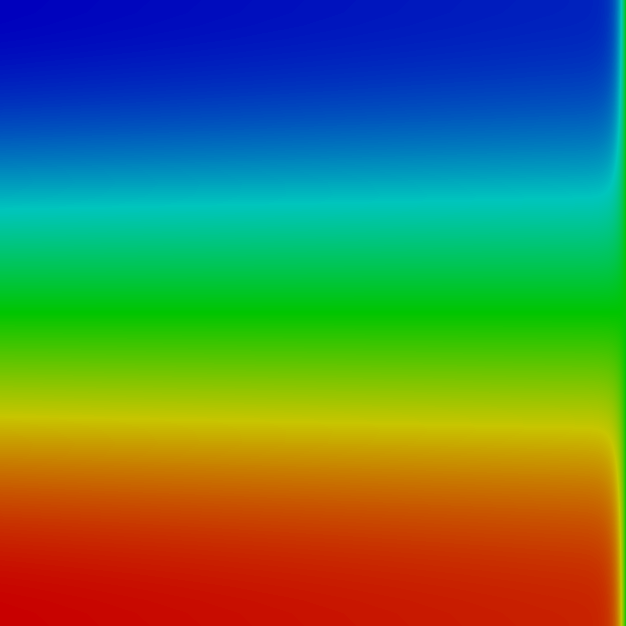
\includegraphics[width=0.5\textwidth]{figs/Erickson/exact.png}
\caption{Erickson-Johnson exact solution}
\label{fig:erickson}
\end{figure}

\begin{figure}[p]
\centering
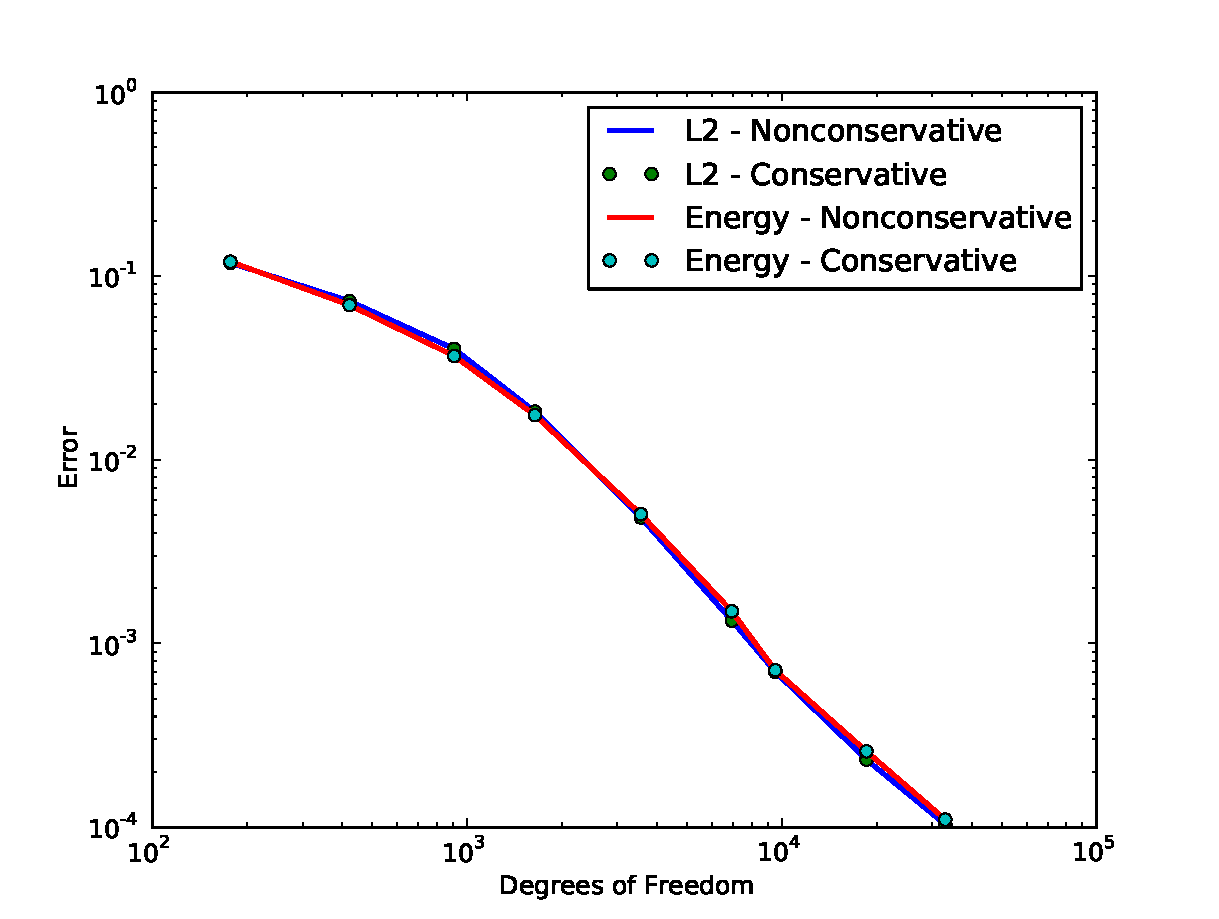
\includegraphics[width=0.7\textwidth]{figs/Erickson/modifiedError.pdf}
\caption{Error in Erickson-Johnson solutions}
\label{fig:ericksonError}
\end{figure}

\begin{figure}[h!]
\centering
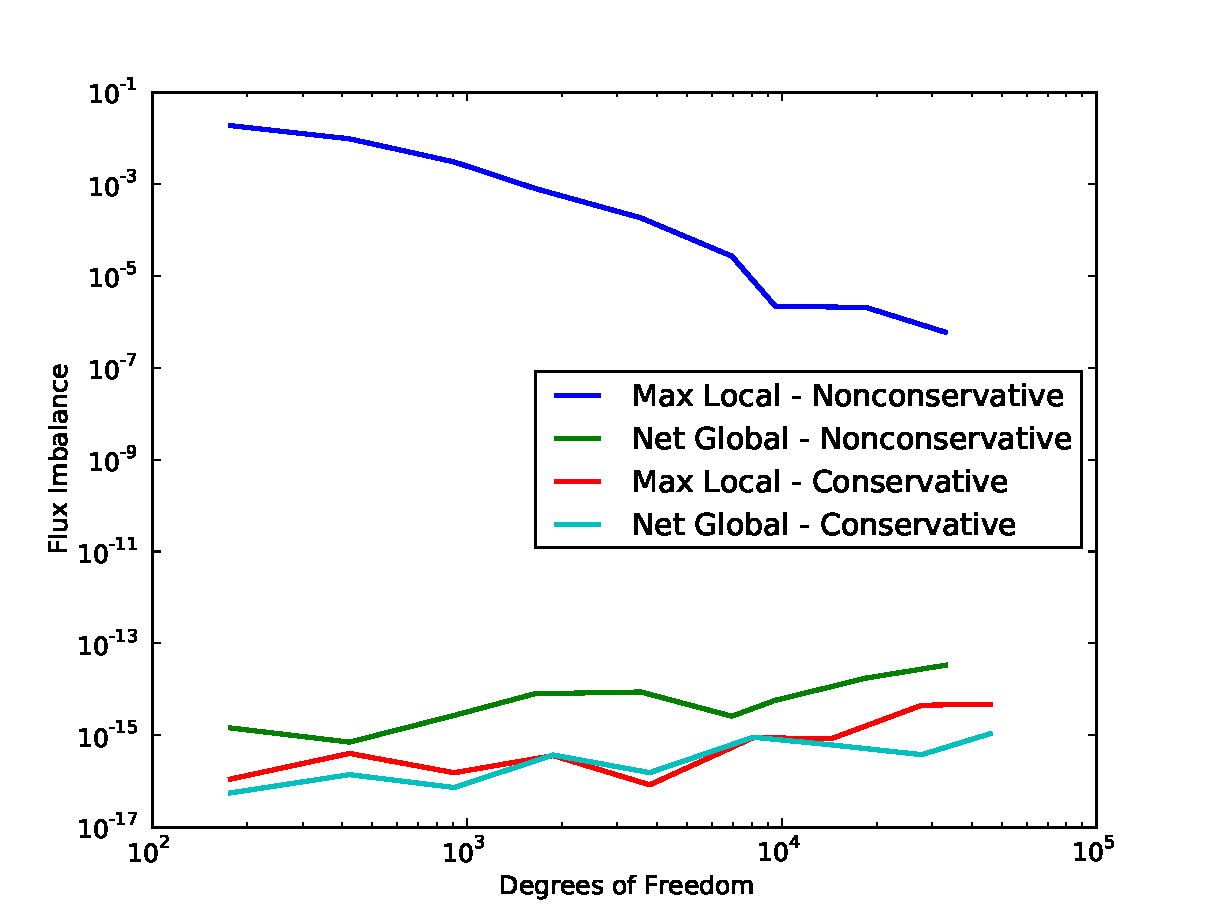
\includegraphics[width=0.7\textwidth]{figs/Erickson/modifiedFlux.pdf}
\caption{Flux imbalance in Erickson-Johnson solutions}
\label{fig:ericksonFlux}
\end{figure}

\subsubsection{Vortex Problem}
This problem models a mildly diffusive vortex convecting fluid in a circle. We
deal with domain $\Omega=[-1,1]^2$, with $\epsilon=10^{-4}$, and
$\bfbeta=(-y,x)^T$. Note that $\bfbeta=\mathbf{0}$ at the domain center. We have an
inflow boundary condition when $\bfbeta\cdot\mathbf{n}<0$, in which case we set
$\hat t=\bfbeta\cdot\mathbf{n}\cdot u_0$ where
$u_0=\frac{\sqrt{x^2+y^2}-1}{\sqrt{2}-1}$ which will vary from 0 at the center
of boundary edges to 1 at corners. We don't enforce an outflow boundary.
Results and flux imbalance are shown in Figure~\ref{fig:vortex} and Figure~\ref{fig:vortex_flux}.

\begin{figure}[p]
\centering
\begin{subfigure}[t]{0.45\textwidth}
\centering
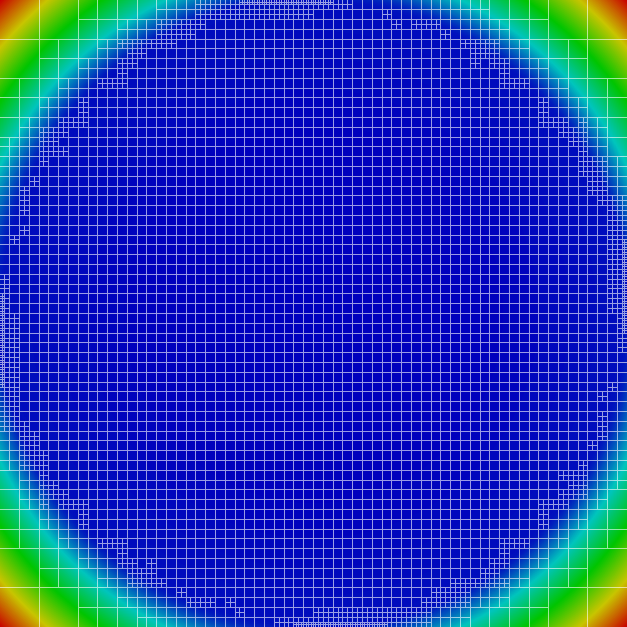
\includegraphics[width=\textwidth]{figs/Vortex/modified6nc.png}
\caption{Nonconservative}
\label{fig:vortexModified6nc}
\end{subfigure}
\begin{subfigure}[t]{0.45\textwidth}
\centering
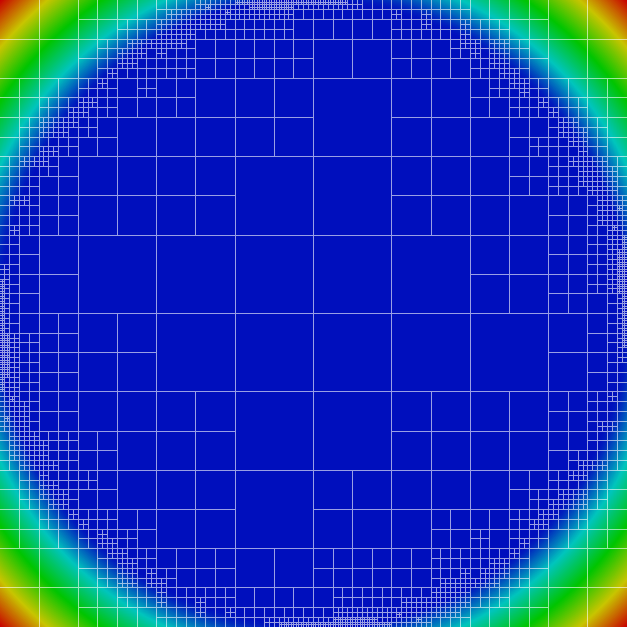
\includegraphics[width=\textwidth]{figs/Vortex/modified6c.png}
\caption{Conservative}
\label{fig:vortexModified6c}
\end{subfigure}
\caption{Vortex problem after 6 refinements}
\label{fig:vortex}
\end{figure}

\begin{figure}[p]
\centering
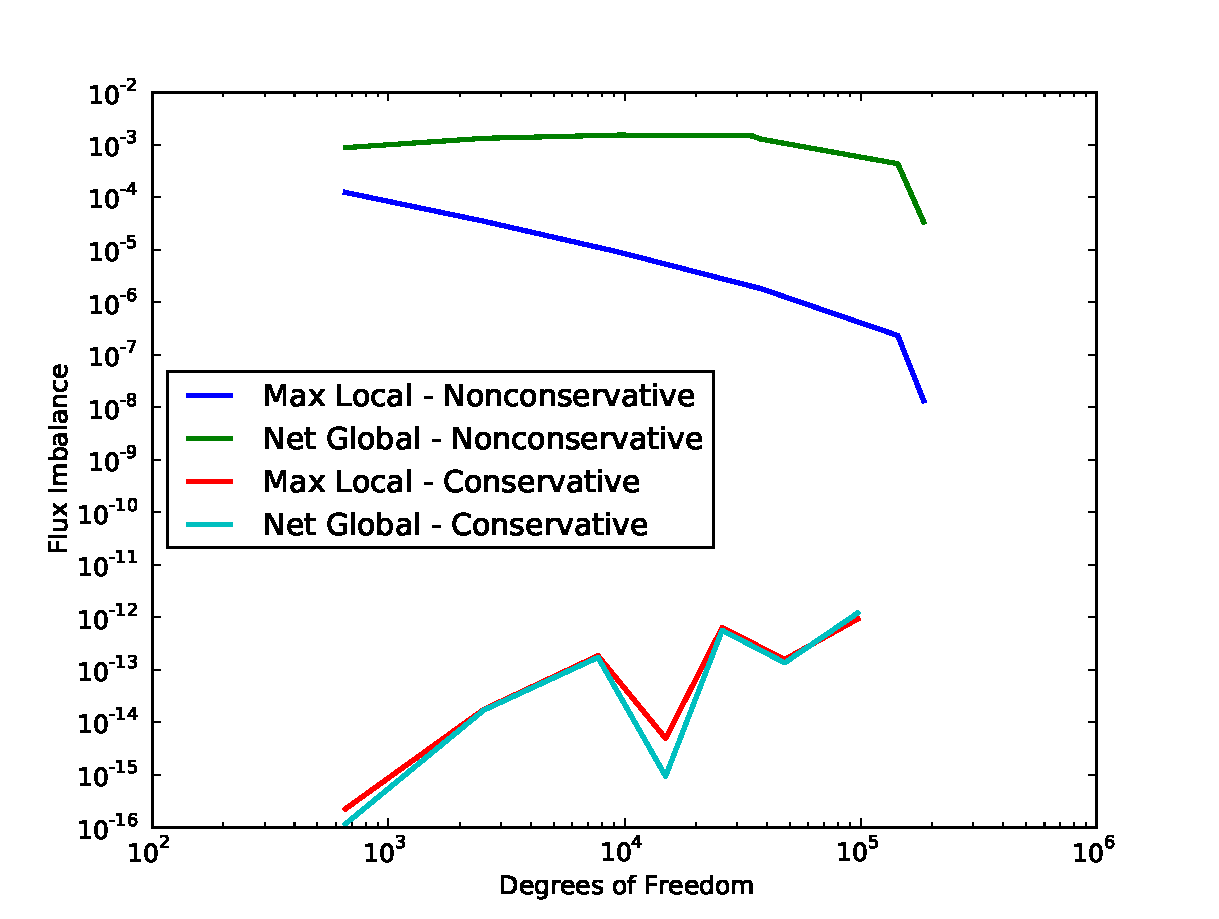
\includegraphics[width=0.7\textwidth]{figs/Vortex/modifiedFlux.pdf}
\caption{Flux imbalance in vortex solutions}
\label{fig:vortex_flux}
\end{figure}

\subsubsection{Discontinuous Source Problem}
Here, $\bfbeta=(0.5,1)^T/\sqrt{1.25}$, and we have a discontinuous source term
such that $f=1$ when $y\ge2x$ and $f=-1$ when $y<2x$. We apply boundary
conditions of $\hat t=0$ on the inflow and $\hat u=0$ on the outflow. Contrary
to the other problems discussed, the solution for this problem does not range
from zero to one. Rather, the colorbar in Figure \ref{fig:discontinuous} is
scaled to  $[-1.110,0.889]$.
Flux imbalance is shown in Figure~\ref{fig:discontinuous_flux}.

\begin{figure}[p]
\centering
\begin{subfigure}[t]{0.45\textwidth}
\centering
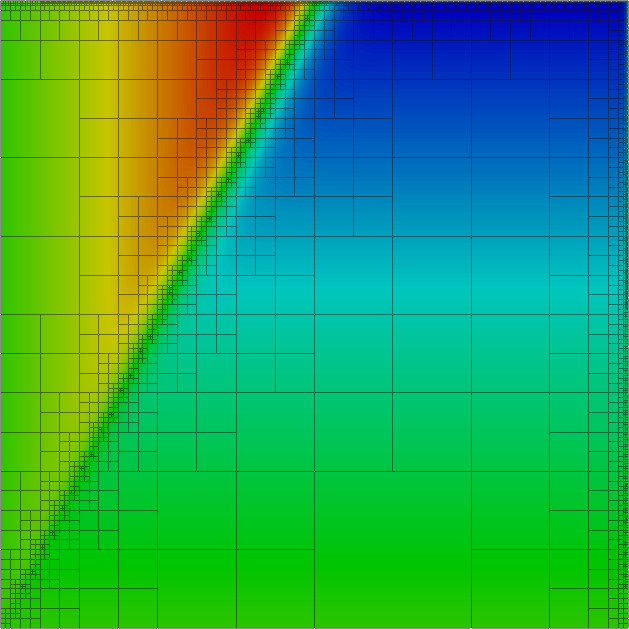
\includegraphics[width=\textwidth]{figs/Discontinuous/modified8nc.png}
\caption{Nonconservative}
\label{fig:discontinuousModified8nc}
\end{subfigure}
\begin{subfigure}[t]{0.45\textwidth}
\centering
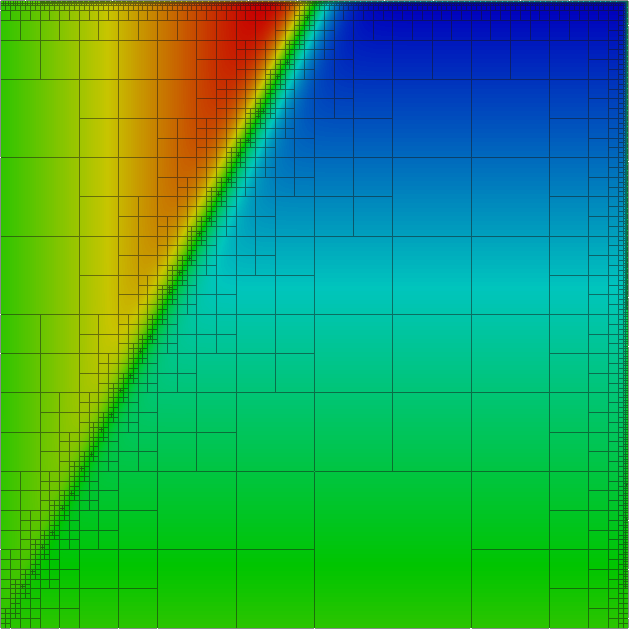
\includegraphics[width=\textwidth]{figs/Discontinuous/modified8c.png}
\caption{Conservative}
\label{fig:discontinuousModified8c}
\end{subfigure}
\caption{Discontinuous source problem after 8 refinements}
\label{fig:discontinuous}
\end{figure}

\begin{figure}[p]
\centering
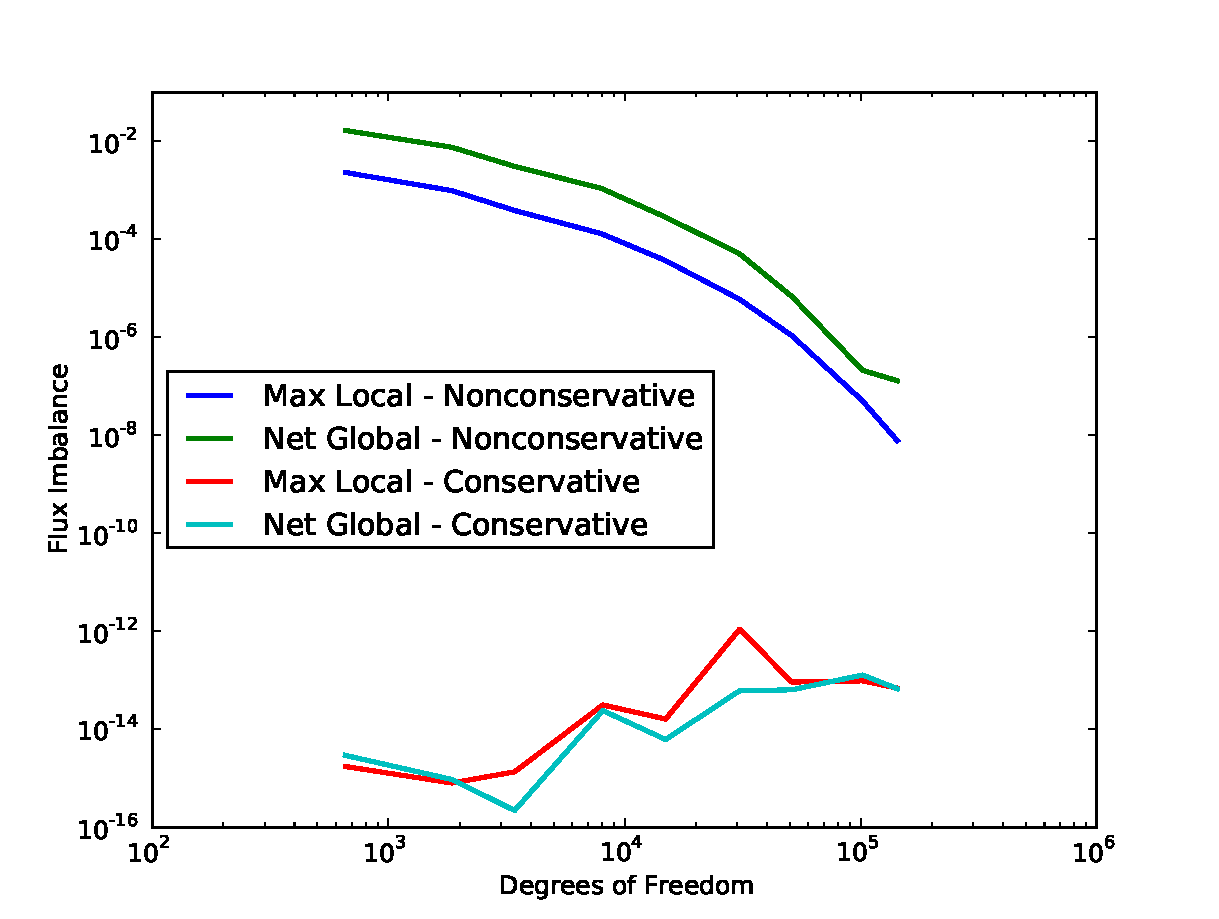
\includegraphics[width=0.7\textwidth]{figs/Discontinuous/modifiedFlux.pdf}
\caption{Flux imbalance in discontinuous source solutions}
\label{fig:discontinuous_flux}
\end{figure}

\subsubsection{Inviscid Burgers' Equation}\label{sec:inviscidBurgers}
This is a standard test problem for Burgers' equation. The domain is a unit
square. We assign boundary conditions $\hat t=-(1-2x)$ on the bottom, $\hat
t=-1/2$ on the left, while $\hat t=1/2$ on the right. Since this is a
hyperbolic equation, there is no need to set a boundary condition on the top.
Results and flux imbalance are shown in Figure~\ref{fig:burgers} and Figure~\ref{fig:burgers_flux}.

\begin{figure}[p]
\centering
\begin{subfigure}[t]{0.45\textwidth}
\centering
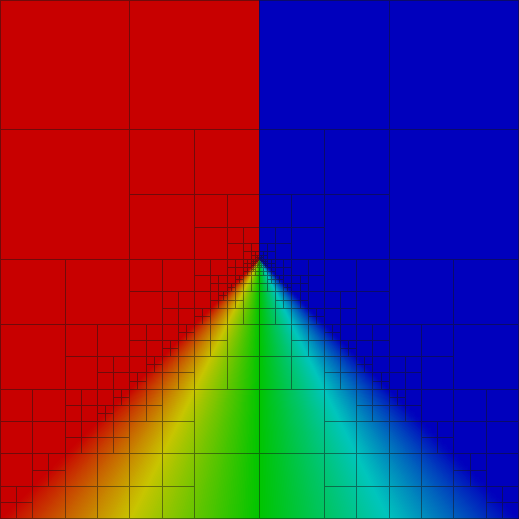
\includegraphics[width=\textwidth]{figs/Burgers/graph8nc.png}
\caption{Nonconservative}
\label{fig:burgers8nc}
\end{subfigure}
\begin{subfigure}[t]{0.45\textwidth}
\centering
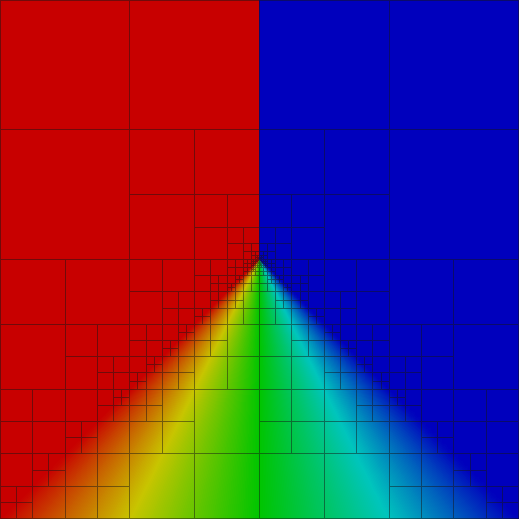
\includegraphics[width=\textwidth]{figs/Burgers/graph8c.png}
\caption{Conservative}
\label{fig:burgers8c}
\end{subfigure}
\caption{Burgers' problem after 8 refinements}
\label{fig:burgers}
\end{figure}

\begin{figure}[p]
\centering
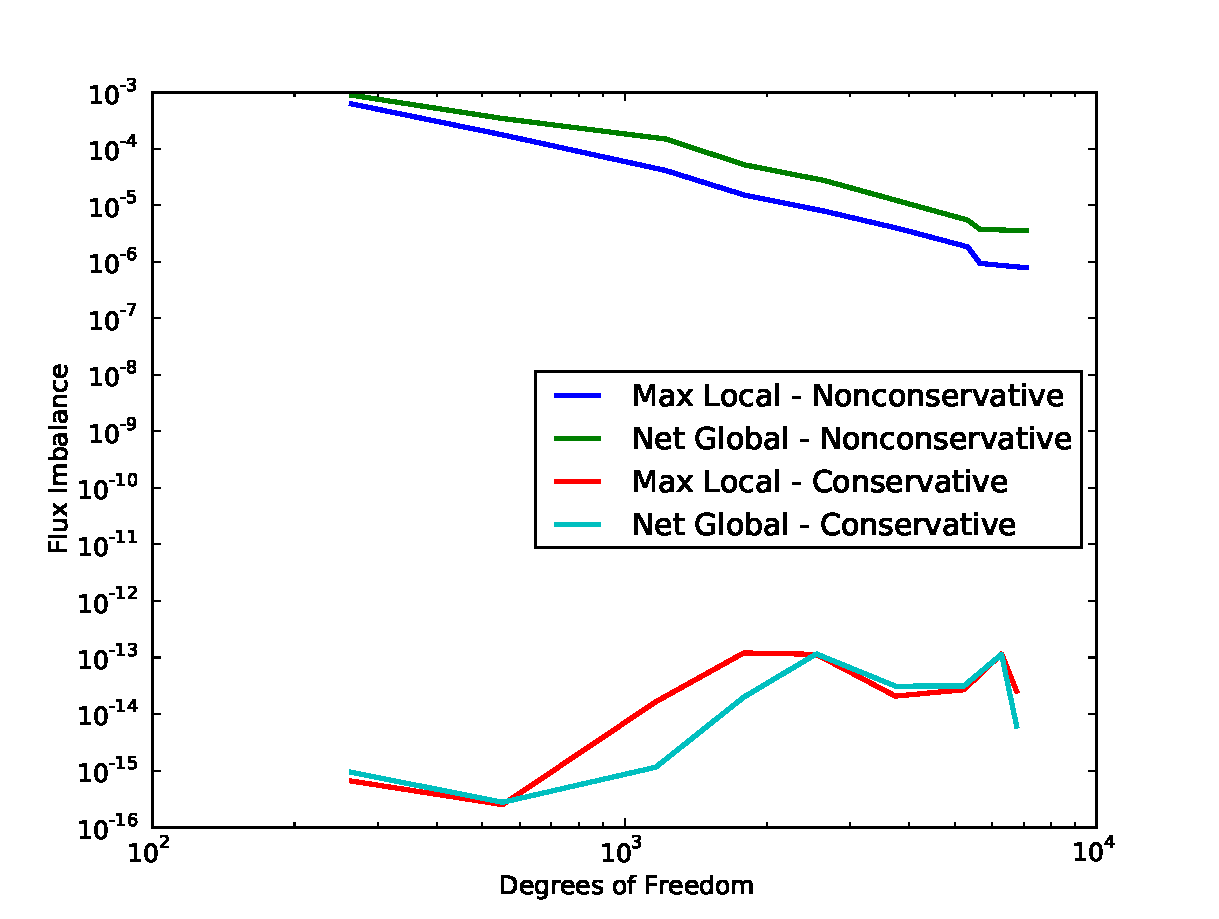
\includegraphics[width=0.7\textwidth]{figs/Burgers/graphFlux.pdf}
\caption{Flux imbalance in Burgers' solutions}
\label{fig:burgers_flux}
\end{figure}

\subsubsection{Stokes Flow Around a Cylinder}\label{sec:stokesCylinder}
This is a common problem used to stress-test local conservation properties of
least squares finite element methods. Since DPG can be viewed as a generalized
least squares methods\cite{DPGOverview}, we might expect it to struggle with
this problem as well. The problem domain is detailed in
Figure~\ref{fig:stokesCylinderDomain} with inlet and outlet velocity profiles
\[
\bfu_{in}=\bfu_{out}=\vecttwo{(1-y)(1+y)}{0}\,,
\]
and zero flow on the cylinder and at the top and bottom walls. We use $\mu=$
with both Stokes problems and set velocity boundary conditions on $\hat\bfu$.

Bochev \etal~\cite{Bochev2010} run this test with both $r=0.6$ and $r=0.9$; we
repeat the same experiments with standard and conservative DPG methods
starting from the very coarse meshes shown in Figure~\ref{fig:stokesMesh}
while adaptively refining toward a resolved solution. The extreme pressure
gradient in the $r=0.9$ case obviously makes local conservation more
challenging.

We measure mass loss more directly in these two Stokes problems. Because
fluid enters and leaves the domain only through the inlet and outlet
boundaries, we should be able to integrate the mass flux over any
cross-section of the mesh and get the same value. Unfortunately, it is not
mathematically well-defined to take line integrals of our field variables which only
live in $L^2$. We can however integrate the trace and flux variables over element boundaries.
This carries the unfortunate limitation that we can only measure mass loss
where there is a clear vertical mesh line. We therefore pick integration lines
from the initial coarse mesh and measure the mass flux after each adaptive refinement
step. The percent mass loss is thus
\[
\%m_{loss}=\frac{\int_{\Gamma_{in}}\bfu\cdot\bfn_{in}d\ell-\int_S\bfu\cdot\bfn_Sd\ell}
{\int_{\Gamma_{in}}\bfu\cdot\bfn_{in}d\ell}\times100,
\]
where $S$ is some vertical mesh line.
Results and mass loss are shown in Figures~\ref{fig:stokesCylinder}~-~\ref{fig:stokesCylinder9MassLoss}.

\begin{figure}[p]
\centering
\begin{tikzpicture}[line cap=round,line join=round,>=triangle 45,x=2.5cm,y=2.5cm]
\clip(-1.97,-1.48) rectangle (3.39,1.55);
\draw(0,0) circle (1.5cm);
\draw (-1,-1)-- (3,-1);
\draw (3,1)-- (3,-1);
\draw (-1,1)-- (3,1);
\draw (-1,1)-- (-1,-1);
\draw (0,0)-- (.3,0.5196);
\draw (0.12,0.29) node[anchor=north west] {r};
\draw (-1.3,-1.0) node[anchor=north west] {-1.0};
\draw (-1.3,1.15) node[anchor=north west] {1.0};
\draw (-1.3,0.0) node[anchor=north west] {$u_{in}$};
\draw (0.6,0.0) node[anchor=north west] {$u_{cyl}$};
\draw (3.0,-1.0) node[anchor=north west] {3.0};
\draw (3.0,0.0) node[anchor=north west] {$u_{out}$};
\draw (0.9,-1.03) node[anchor=north west] {$u_{wall}$};
\draw (0.9,1.17) node[anchor=north west] {$u_{wall}$};
\end{tikzpicture}
\caption{Stokes cylinder domain}
\label{fig:stokesCylinderDomain}
\end{figure}

\begin{figure}[p]
\centering
\begin{subfigure}[t]{0.5\textwidth}
\centering
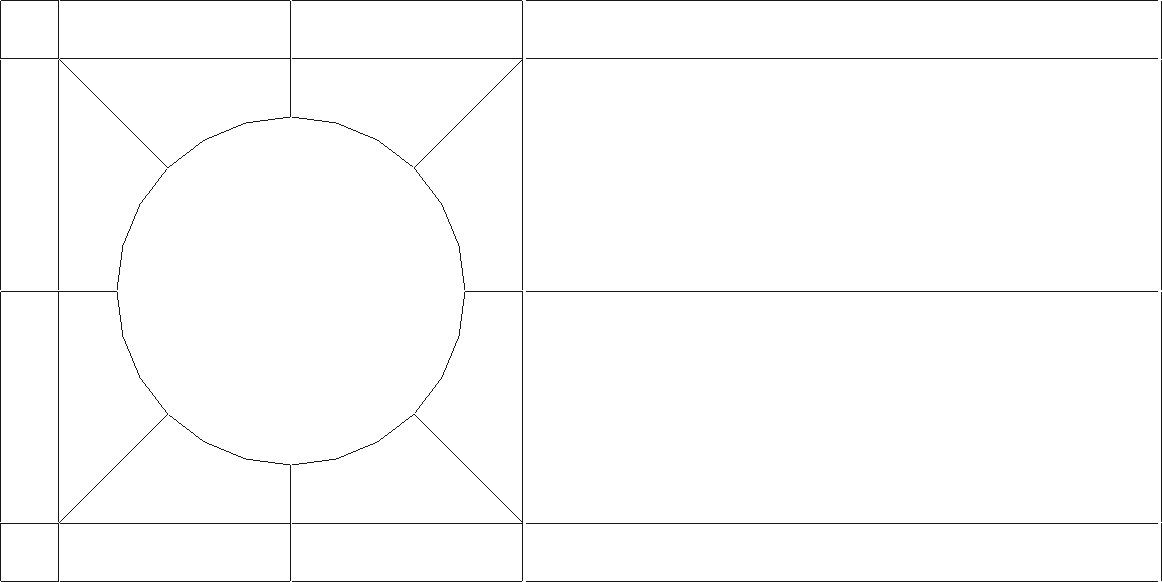
\includegraphics[width=\textwidth]{figs/StokesCylinder/mesh6_0.png}
\caption{Mesh for $r=0.6$}
\label{fig:stokesMesh6}
\end{subfigure}
\begin{subfigure}[t]{0.5\textwidth}
\centering
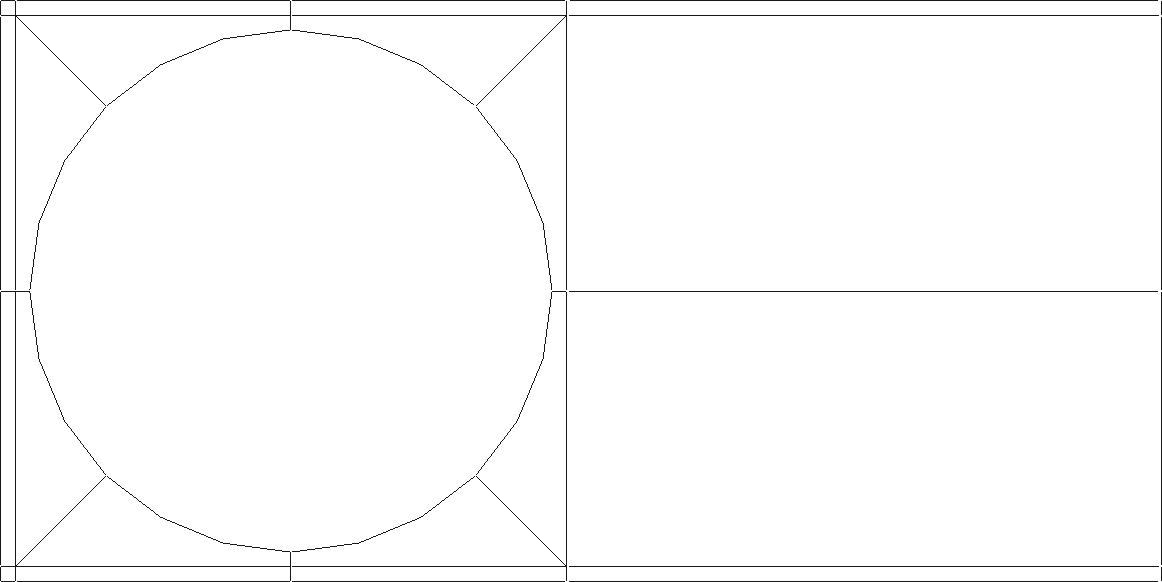
\includegraphics[width=\textwidth]{figs/StokesCylinder/mesh9_0.png}
\caption{Mesh for $r=0.9$}
\label{fig:stokesMesh9}
\end{subfigure}
\caption{Initial mesh for Stokes flow over a cylinder}
\label{fig:stokesMesh}
\end{figure}

\begin{figure}[p]
\centering
\begin{subfigure}[t]{0.45\textwidth}
\centering
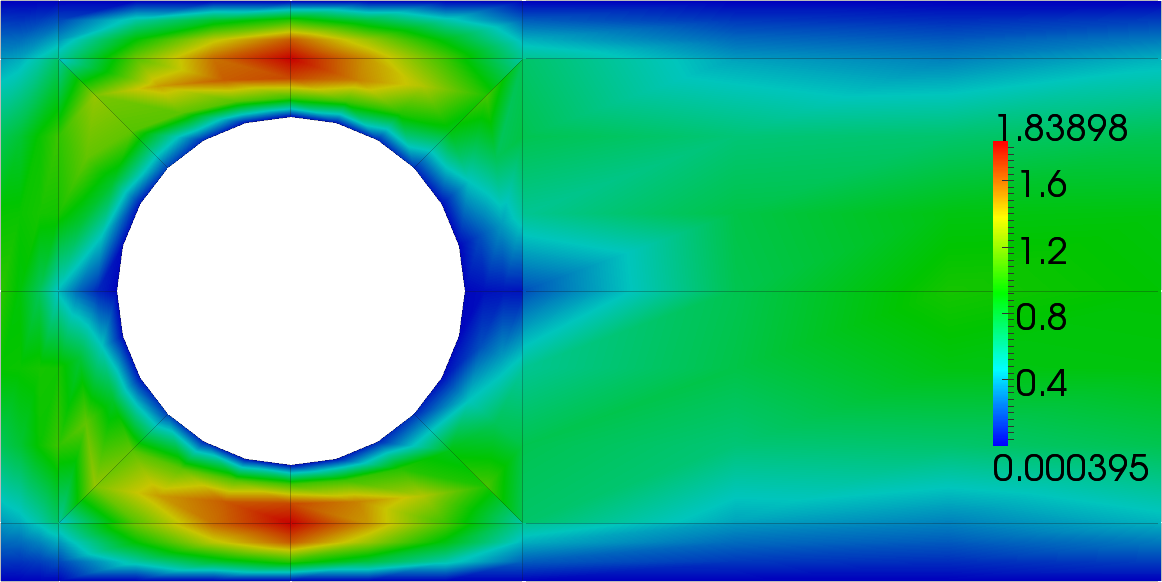
\includegraphics[width=\textwidth]{figs/StokesCylinder/umag6_NC0.png}
\caption{Nonconservative on initial mesh with $r=0.6$}
\label{fig:stokesCylinder6NC0}
\end{subfigure}
\begin{subfigure}[t]{0.45\textwidth}
\centering
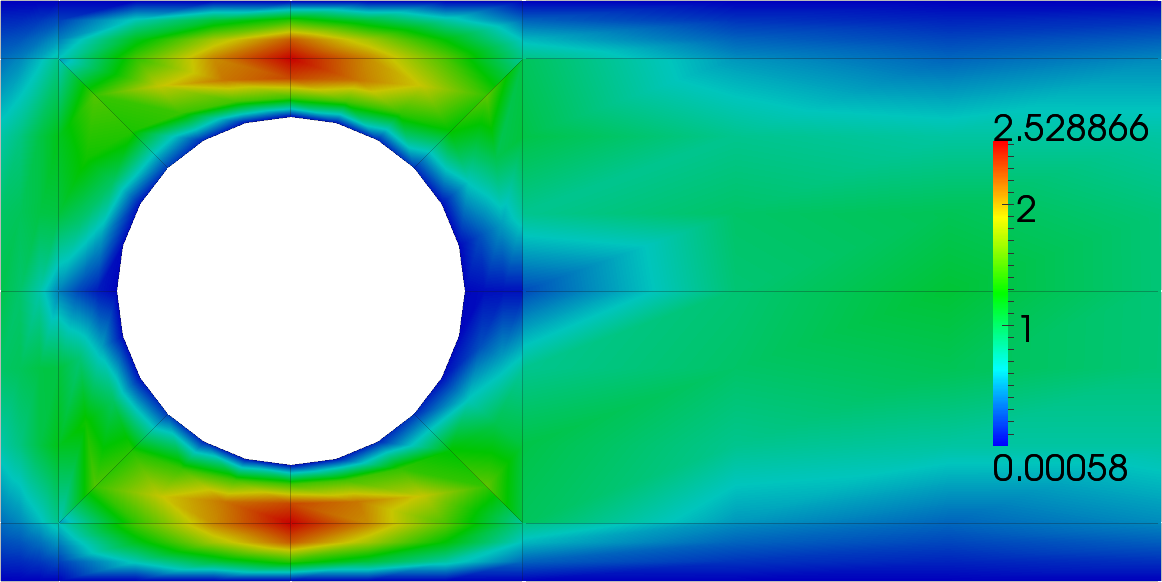
\includegraphics[width=\textwidth]{figs/StokesCylinder/umag6_C0.png}
\caption{Conservative on initial mesh with $r=0.6$}
\label{fig:stokesCylinder6C0}
\end{subfigure}
\begin{subfigure}[t]{0.45\textwidth}
\centering
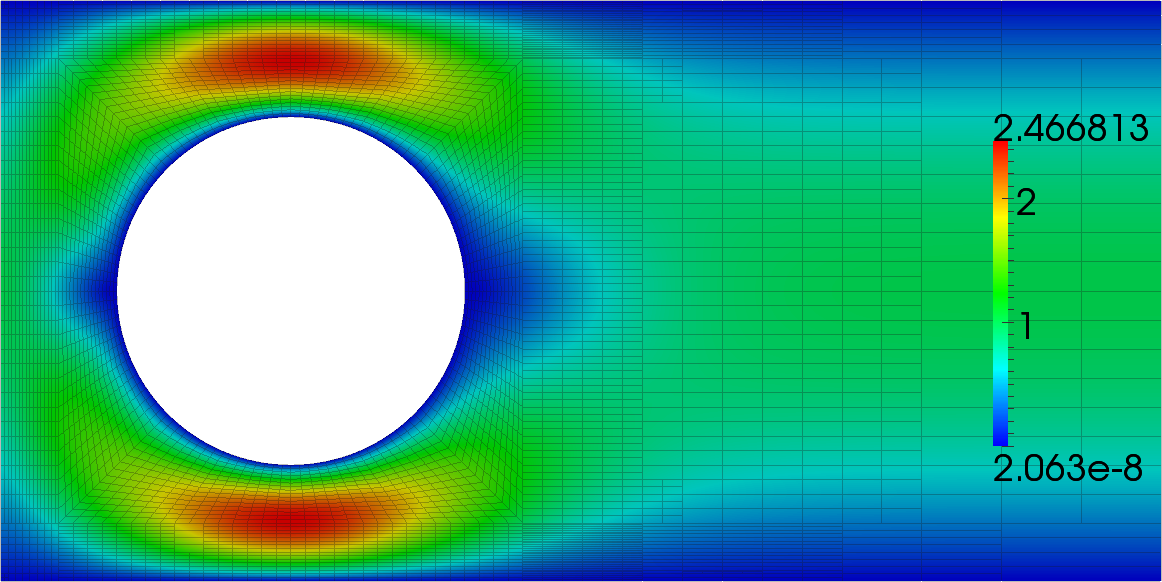
\includegraphics[width=\textwidth]{figs/StokesCylinder/umag6_NC6.png}
\caption{Nonconservative after 6 refinements with $r=0.6$}
\label{fig:stokesCylinder6NC6}
\end{subfigure}
\begin{subfigure}[t]{0.45\textwidth}
\centering
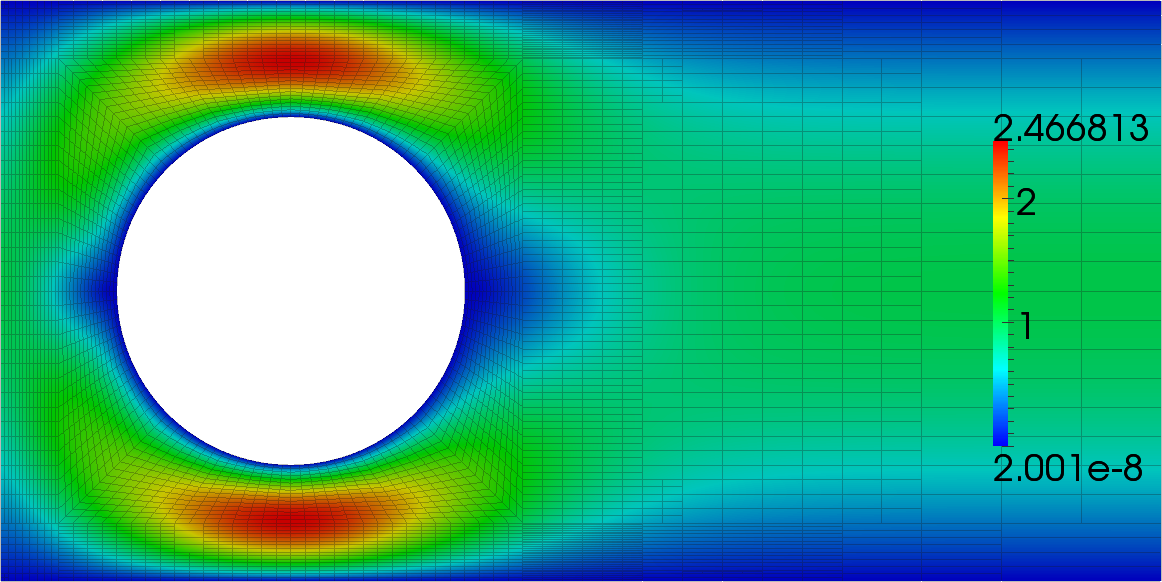
\includegraphics[width=\textwidth]{figs/StokesCylinder/umag6_C6.png}
\caption{Conservative after 6 refinements with $r=0.6$}
\label{fig:stokesCylinder6C6}
\end{subfigure}
\begin{subfigure}[t]{0.45\textwidth}
\centering
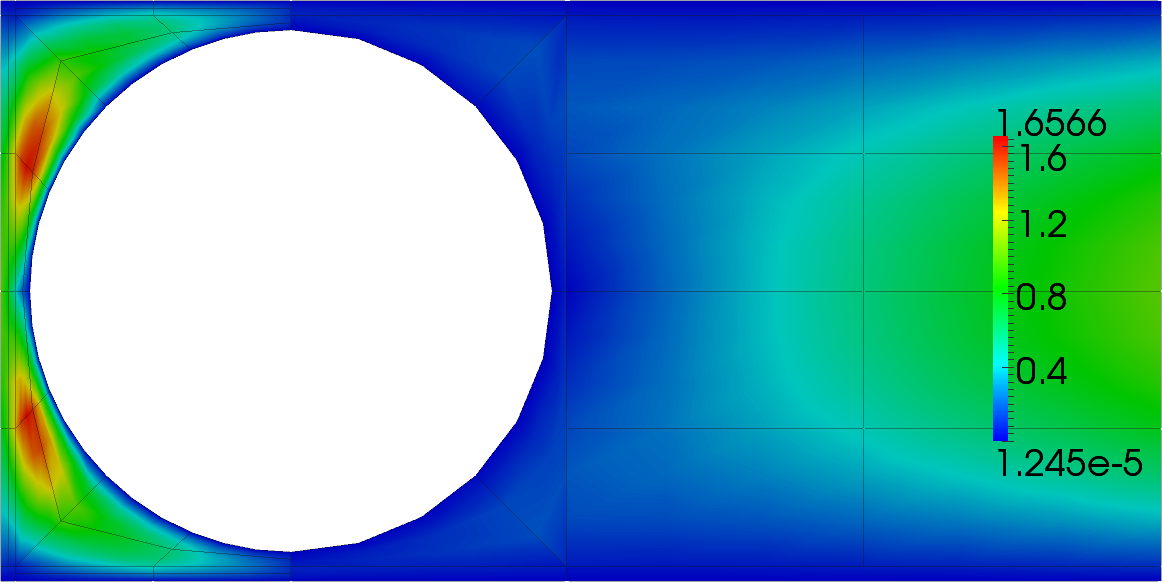
\includegraphics[width=\textwidth]{figs/StokesCylinder/umag9_NC1.png}
\caption{Nonconservative after 1 refinement with $r=0.9$}
\label{fig:stokesCylinder9NC1}
\end{subfigure}
\begin{subfigure}[t]{0.45\textwidth}
\centering
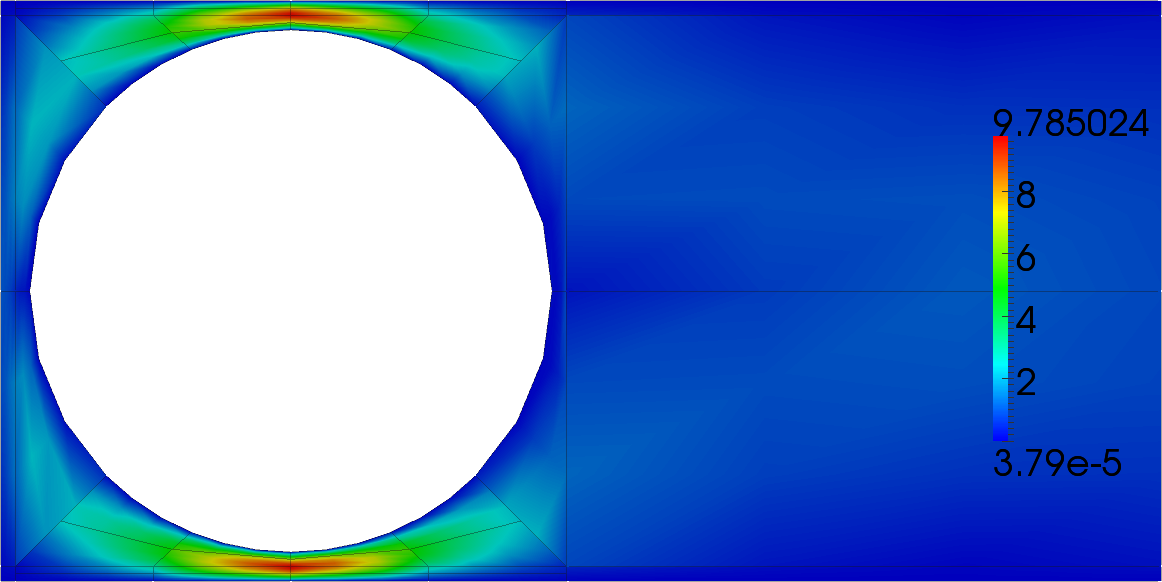
\includegraphics[width=\textwidth]{figs/StokesCylinder/umag9_C1.png}
\caption{Conservative after 1 refinement with $r=0.9$}
\label{fig:stokesCylinder9C1}
\end{subfigure}
\begin{subfigure}[t]{0.45\textwidth}
\centering
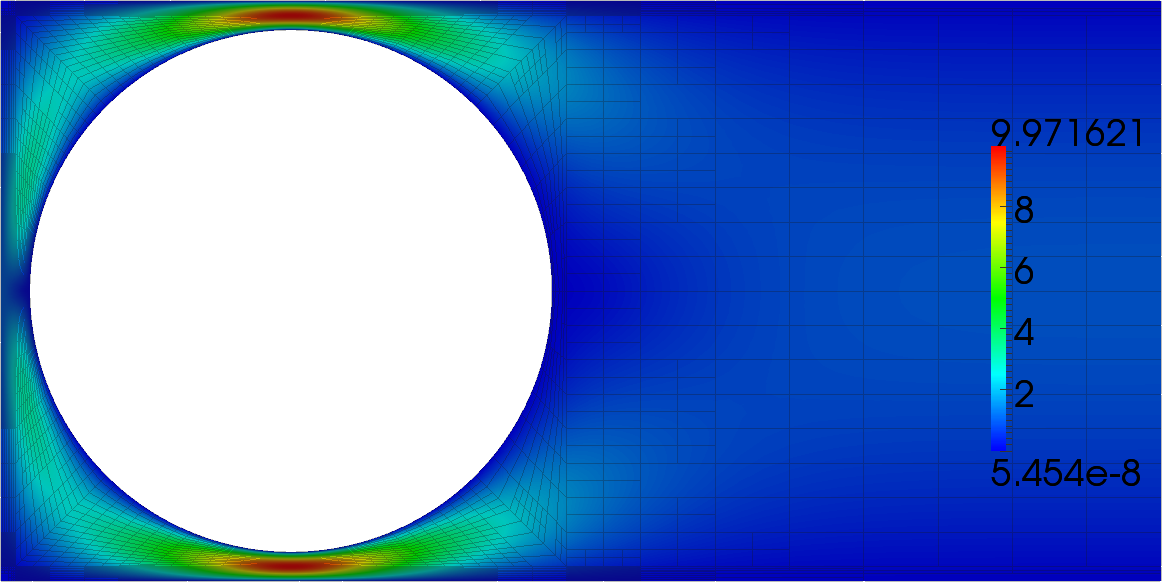
\includegraphics[width=\textwidth]{figs/StokesCylinder/umag9_NC6.png}
\caption{Nonconservative after 6 refinements with $r=0.9$}
\label{fig:stokesCylinder9NC6}
\end{subfigure}
\begin{subfigure}[t]{0.45\textwidth}
\centering
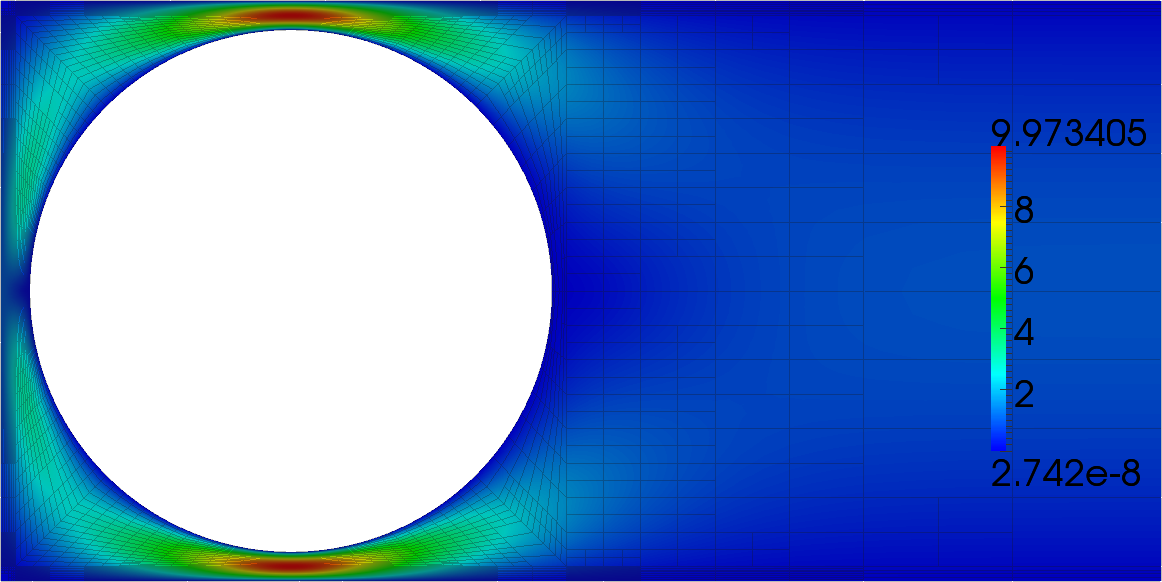
\includegraphics[width=\textwidth]{figs/StokesCylinder/umag9_C6.png}
\caption{Conservative after 6 refinements with $r=0.9$}
\label{fig:stokesCylinder9C6}
\end{subfigure}
\caption{Stokes flow around a cylinder - velocity magnitude}
\label{fig:stokesCylinder}
\end{figure}

\begin{figure}[p]
\centering
\begin{subfigure}[t]{0.7\textwidth}
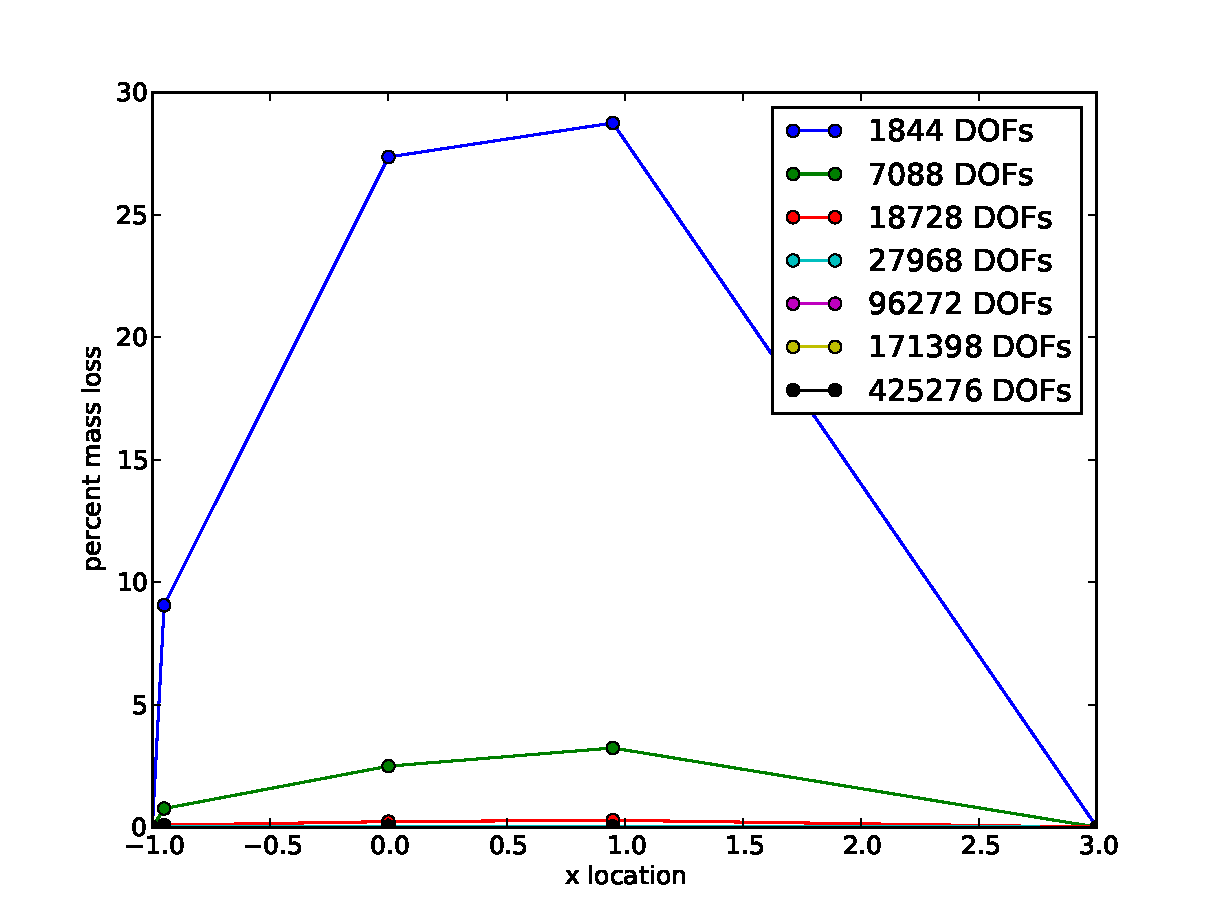
\includegraphics[width=\textwidth]{figs/StokesCylinder/MassLoss6_NC.pdf}
\caption{Nonconservative}
\label{fig:stokesCylinder6MassLossNC}
\end{subfigure}
\begin{subfigure}[t]{0.7\textwidth}
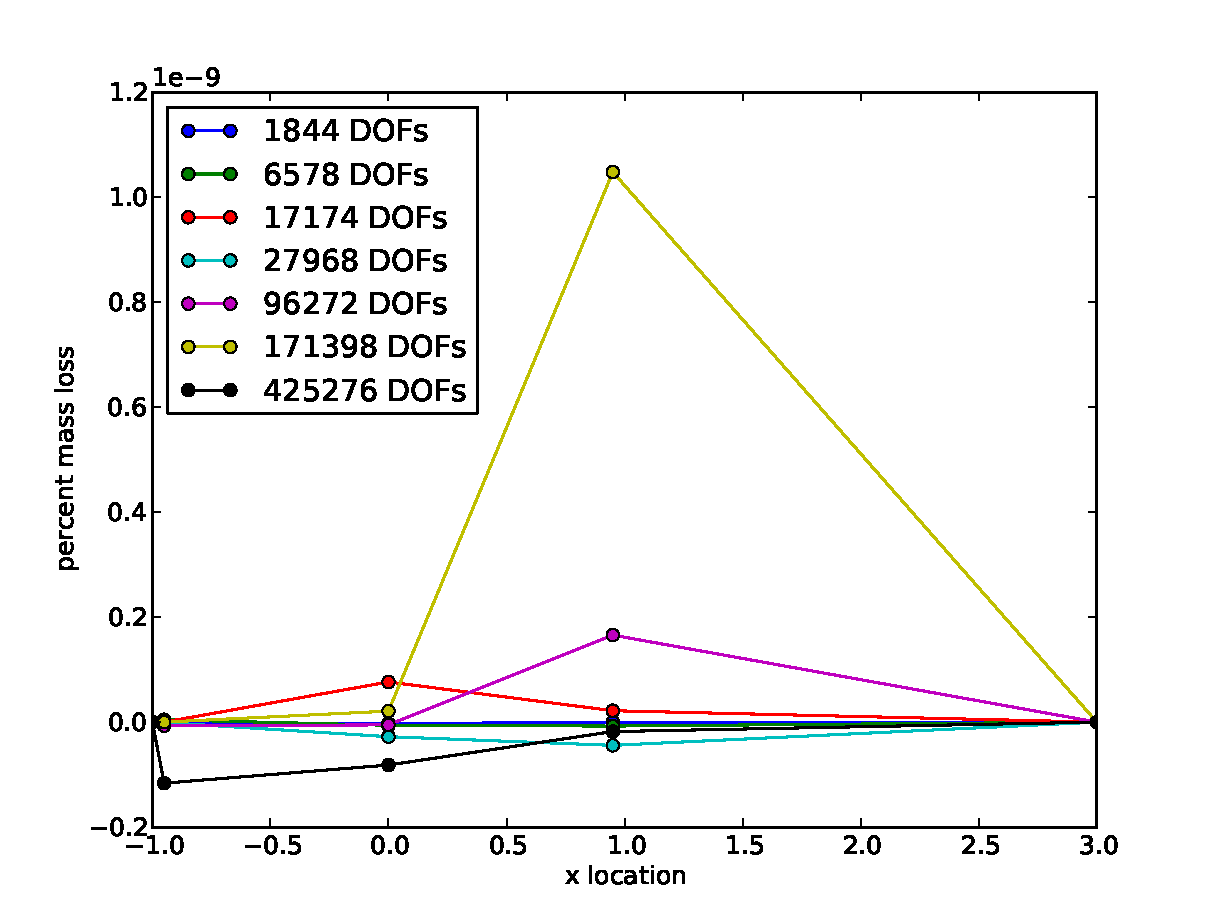
\includegraphics[width=\textwidth]{figs/StokesCylinder/MassLoss6_C.pdf}
\caption{Conservative}
\label{fig:stokesCylinder6MassLossC}
\end{subfigure}
\caption{Mass loss in Stokes flow around a cylinder of radius $0.6$}
\label{fig:stokesCylinder6MassLoss}
\end{figure}

\begin{figure}[p]
\centering
\begin{subfigure}[t]{0.7\textwidth}
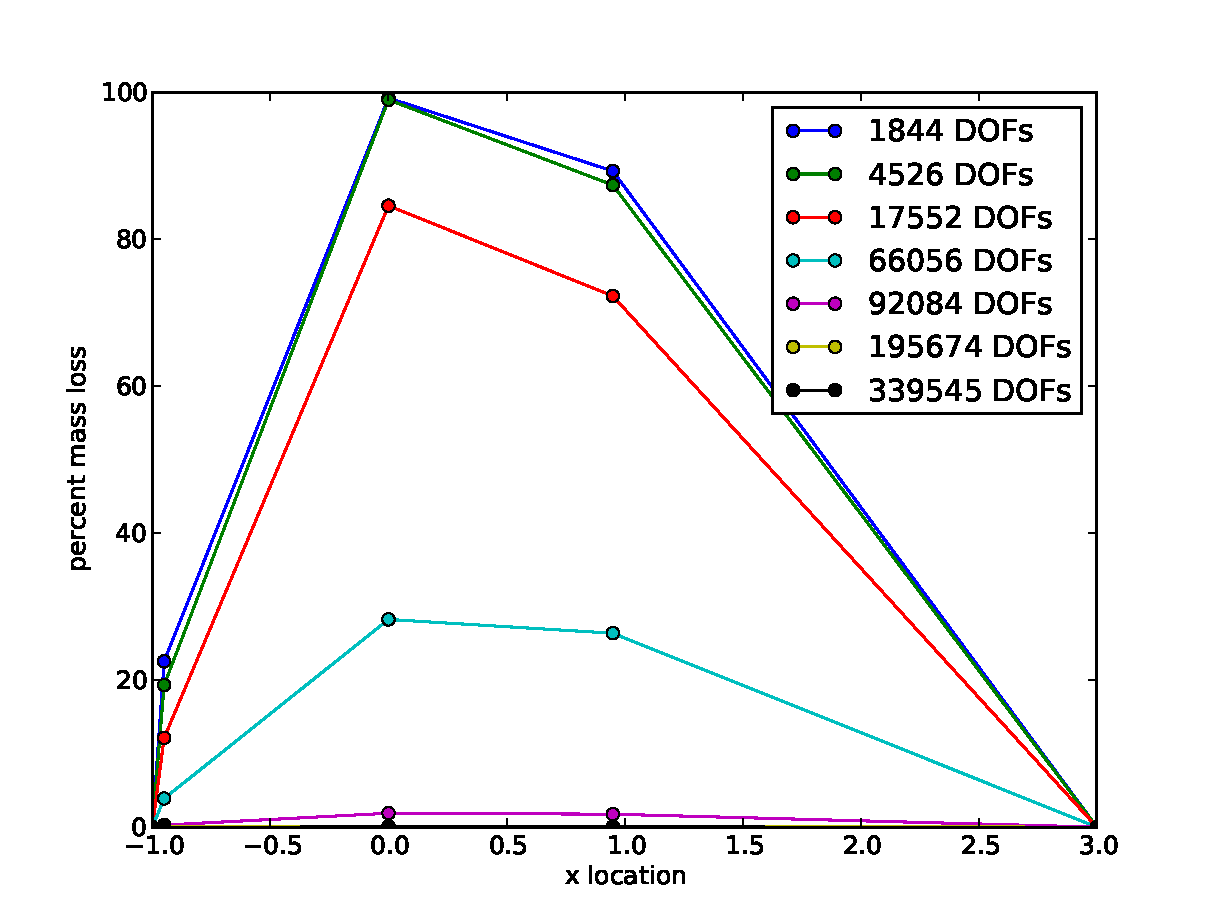
\includegraphics[width=\textwidth]{figs/StokesCylinder/MassLoss9_NC.pdf}
\caption{Nonconservative}
\label{fig:stokesCylinder9MassLossNC}
\end{subfigure}
\begin{subfigure}[t]{0.7\textwidth}
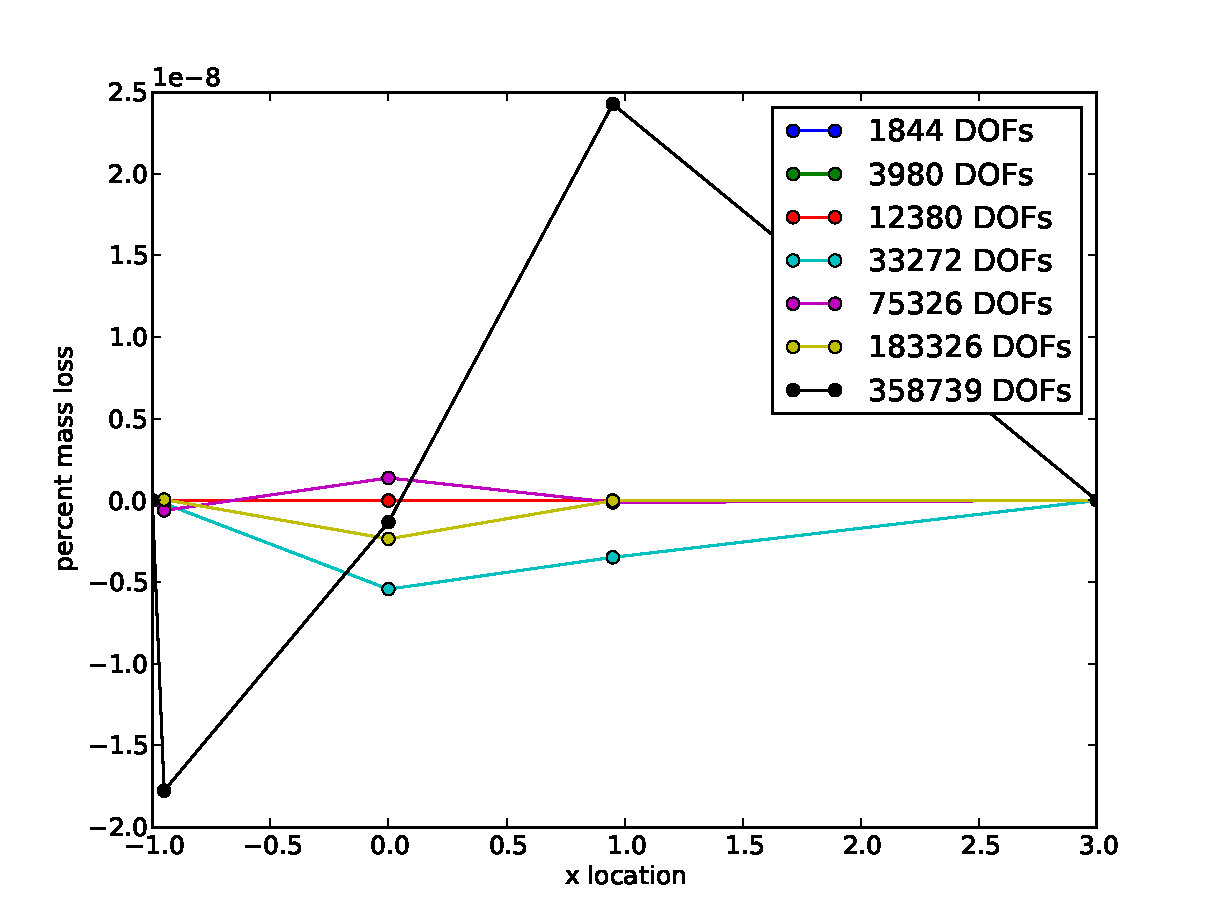
\includegraphics[width=\textwidth]{figs/StokesCylinder/MassLoss9_C.pdf}
\caption{Conservative}
\label{fig:stokesCylinder9MassLossC}
\end{subfigure}
\caption{Mass loss in Stokes flow around a cylinder of radius $0.9$}
\label{fig:stokesCylinder9MassLoss}
\end{figure}

\subsubsection{Stokes Flow Over a Backward Facing Step}\label{sec:stokesStep}
Similarly, least squares methods have historically performed very poorly when
calculating Stokes flow over a backward facing step shown in
Figure~\ref{fig:stokesStepDomain}. The stress singularity at
the reentrant corner seems to destroy local conservation. We
assign parabolic inlet and outlet velocity boundary conditions
\[
\bfu_{in}=\vecttwo{8(y-0.5)(1-y)}{0}
\quad\text{ and }\quad
\bfu_{out}=\vecttwo{y(1-y)}{0}
\]
and zero velocity on all other boundaries. In this problem, we solve with
fourth order field and flux variables, fifth order traces, and sixth order
test functions.
Results and mass loss are shown in Figure~\ref{sec:stokesStep} and Figure~\ref{fig:stokesStepMassLoss}.

\begin{figure}[!h]
\centering
\begin{tikzpicture}[line cap=round,line join=round,>=triangle 45,x=1.3cm,y=1.3cm]
\clip(-0.5,-0.3) rectangle (10.67,2);
\draw [line width=1.0pt] (0,0.5)-- (2,0.5);
\draw [line width=1.0pt] (2,0.5)-- (2,0);
\draw [line width=1.0pt] (10,0)-- (2,0);
\draw [line width=1.0pt] (10,1)-- (10,0);
\draw [line width=1.0pt] (0,1)-- (10,1);
\draw [line width=1.0pt] (0,0.5)-- (0,1);
\draw (-0.6,0.6) node[anchor=north west] {0.5};
\draw (-0.6,1.3) node[anchor=north west] {1.0};
\draw (1.4,0.2) node[anchor=north west] {2.0};
\draw (10.0,0.2) node[anchor=north west] {10.0};
\draw (0.0,0.92) node[anchor=north west] {$u_{in}$};
\draw (10.0,0.7) node[anchor=north west] {$u_{out}$};
\draw (5.0,0.0) node[anchor=north west] {$u_{wall}$};
\draw (5.0,1.35) node[anchor=north west] {$u_{wall}$};
\end{tikzpicture}
\caption{Stokes step domain}
\label{fig:stokesStepDomain}
\end{figure}

\begin{figure}[p]
\centering
\begin{subfigure}[t]{0.7\textwidth}
\centering
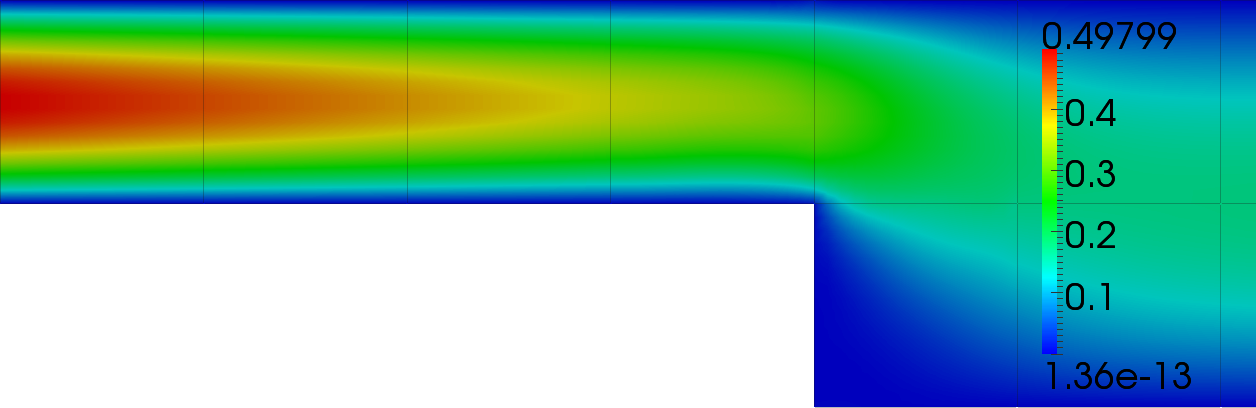
\includegraphics[width=\textwidth]{figs/StokesStep/Quartic_NC0.png}
\caption{Nonconservative on initial mesh}
\end{subfigure}
\begin{subfigure}[t]{0.7\textwidth}
\centering
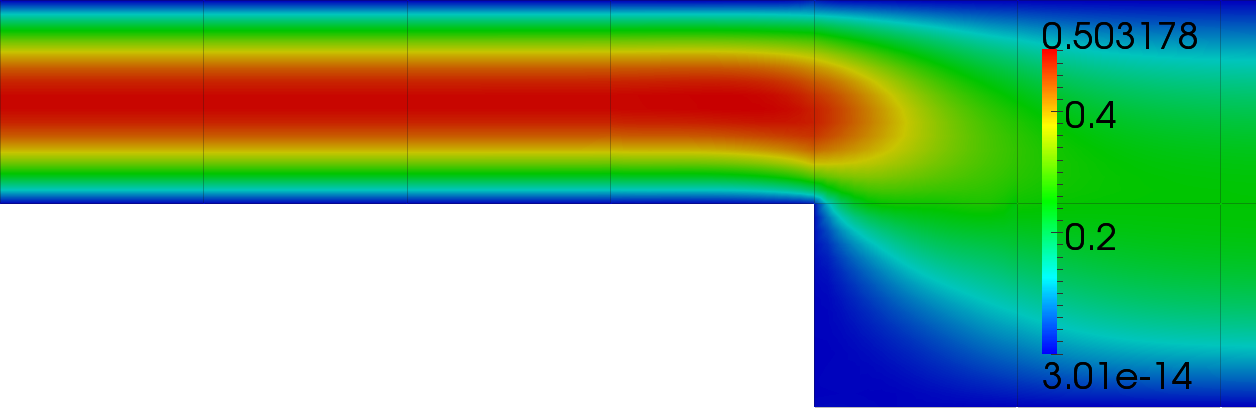
\includegraphics[width=\textwidth]{figs/StokesStep/Quartic_C0.png}
\caption{Conservative on initial mesh}
\end{subfigure}
\begin{subfigure}[t]{0.7\textwidth}
\centering
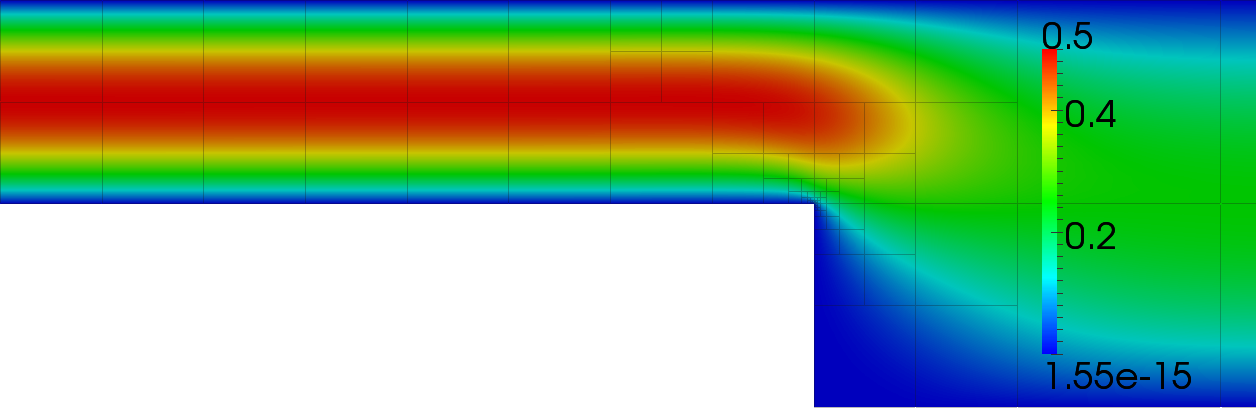
\includegraphics[width=\textwidth]{figs/StokesStep/Quartic_NC8.png}
\caption{Nonconservative after 8 refinement steps}
\label{fig:stokesStepNC}
\end{subfigure}
\begin{subfigure}[t]{0.7\textwidth}
\centering
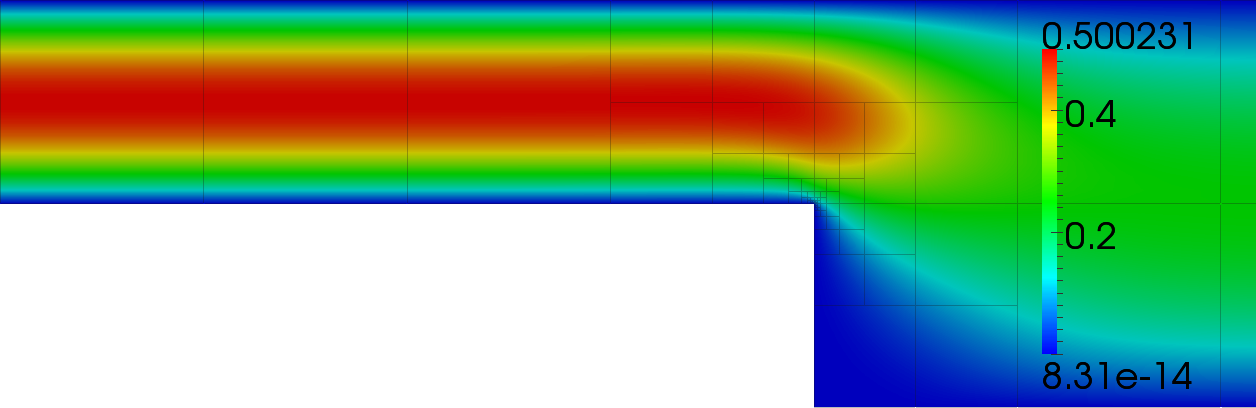
\includegraphics[width=\textwidth]{figs/StokesStep/Quartic_C8.png}
\caption{Conservative after 8 refinement steps}
\label{fig:stokesStepC}
\end{subfigure}
\caption{Stokes backward facing step - velocity magnitude}
\label{fig:stokesStep}
\end{figure}

\begin{figure}[p]
\centering
\begin{subfigure}[t]{0.7\textwidth}
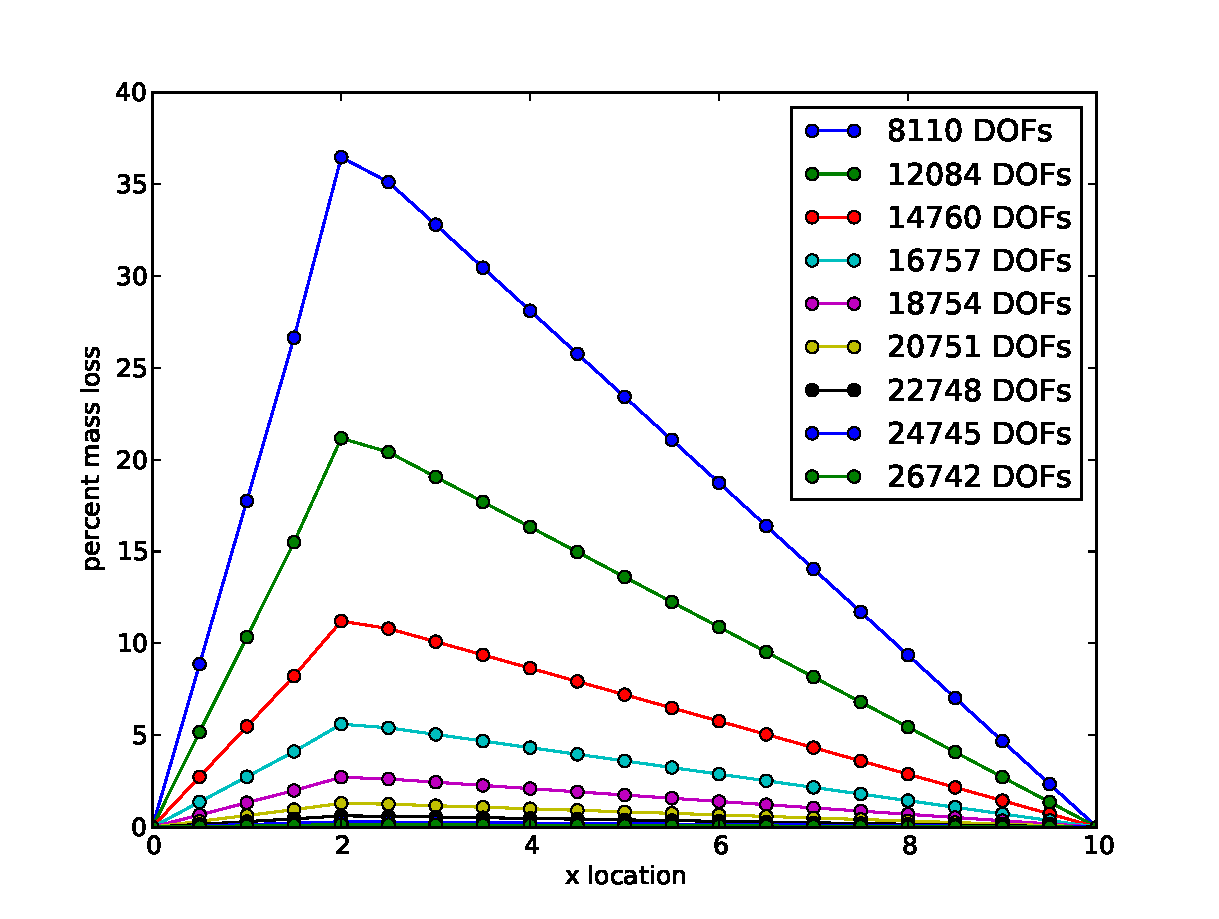
\includegraphics[width=\textwidth]{figs/StokesStep/MassLoss_NC.pdf}
\caption{Nonconservative}
\label{fig:stokesStepMassLossNC}
\end{subfigure}
\begin{subfigure}[t]{0.7\textwidth}
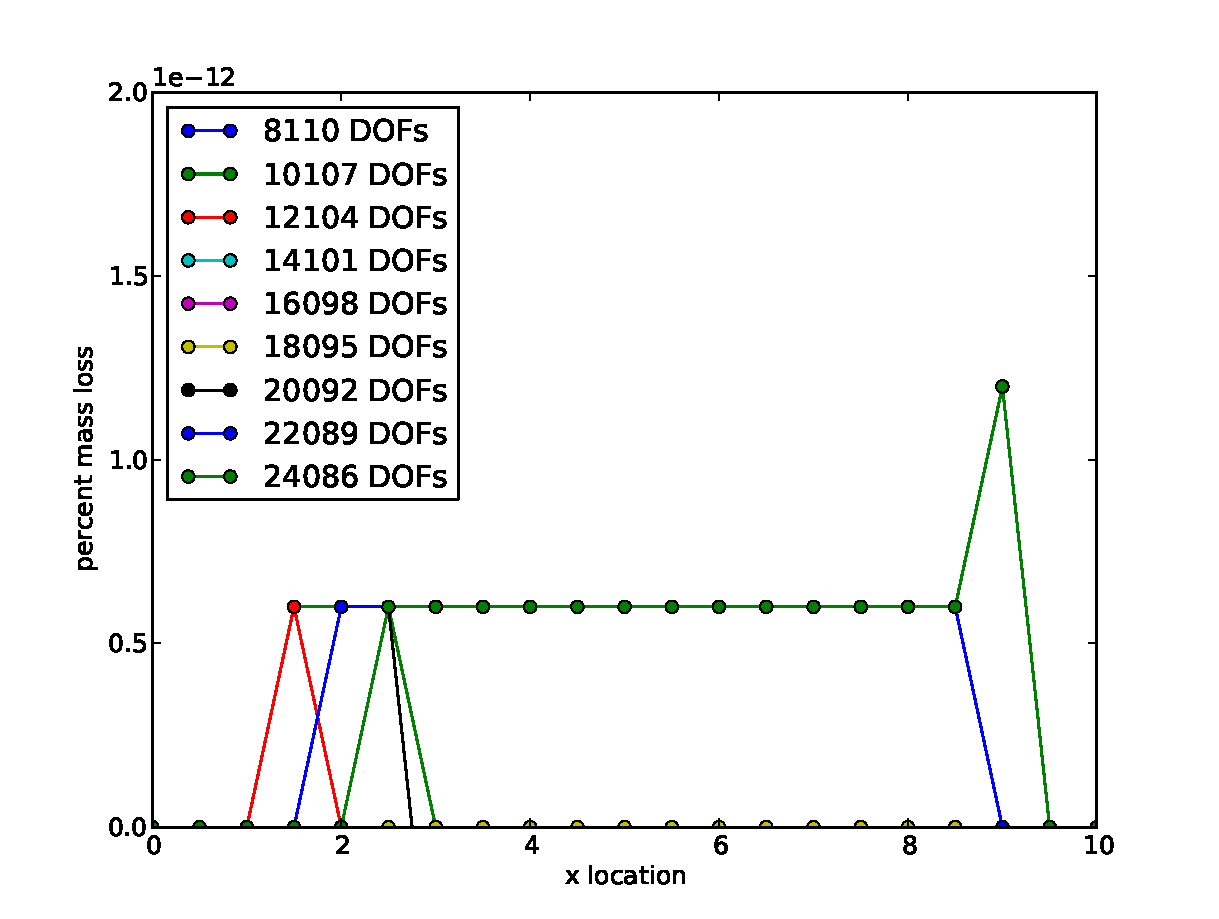
\includegraphics[width=\textwidth]{figs/StokesStep/MassLoss_C.pdf}
\caption{Conservative}
\label{fig:stokesStepMassLossC}
\end{subfigure}
\caption{Mass loss in Stokes backward facing step}
\label{fig:stokesStepMassLoss}
\end{figure}

\subsection{Analysis of Results}\label{sec:problemAnalysis}
\subsubsection{Convection-Diffusion Results}
% Solution quality
The general trend we observe from the results is that the solution quality
of the standard and conservative formulations is nearly identical once
sufficiently resolved.

% Overshoots/undershoots
% Another measure of solution quality is to look at the magnitude of overshoots
% and undershoots in the solution. In most of the convection-diffusion problems considered (barring
% the discontinuous source problem) the exact solution would range exactly
% between 0 and 1. In the resolved solutions, the divergence from these values
% would be negligible, but for the inner layer, in which $\epsilon=10^{-6}$, we
% get overshoots and undershoots along the separation line. For the
% standard formulation, the solution range for $u$ was $[-0.392,1.342]$,
% while the conservative solution range was $[-0.389,1.378]$. This difference is
% easily accounted for by the differences in refinement patterns between the two
% methods.

% Mesh refinements
It is clear when comparing the refinement patterns that the two methods appear
to calculate slightly different error representation functions (which
determine which elements to adaptively refine). Standard DPG minimizes the
error in the energy norm, but the Lagrange multipliers in the conservative
formulation shift the solution slightly, so we should see somewhat higher
error and different elements will get chosen for refinement. The choice of
test norm also plays into this calculation of the error representation
function. As discussed earlier, the conservative formulation allows us to
throw away the $L^2$ term on $v$. The inclusion of this term required certain
assumptions on $\bfbeta$ \cite{ChanHeuerThanhDemkowicz2012} that break down for
the vortex problem, where $\snorm{\bfbeta}\rightarrow 0$ in the center of the domain.
Here, we see the standard method needlessly refines
in the center of the domain where the solution is constant. The conservative
scheme is more discerning about refinements and focuses them where
solution features are changing. In general, though, both methods appear to
follow very similar refinement patterns.

% Mass conservation
It should not come as a surprise that the standard and conservative
solutions match each other so closely. The conservative formulation
enforces local conservation more strictly, but if we examine the flux
imbalance plots, the standard DPG formulation is nearly conservative on its
own -- and appears to become more conservative with refinement. The flux
imbalance of the conservative methods appears to bounce around close to the
machine epsilon (plus a few orders of magnitude). The level of enforcement
appears to creep up with more degrees of freedom, indicating possible
accruement of numerical error.

\subsubsection{Burgers' Results}
Standard and conservative DPG perform nearly identically for the
inviscid Burgers' problem. It is obvious that the Lax-Wendroff condition of
local conservation is a sufficient, but not necessary condition for numerical
solutions to hyperbolic conservation laws. We see the same behavior with the
flux imbalance plots that was so common with convection-diffusion.

\subsubsection{Stokes Results}
The two Stokes problems are the first ones we encounter that stress the local
conservation property of standard DPG. With a cylinder radius of $0.6$,
standard DPG loses nearly 30\% of the mass post-cylinder, but quickly recovers
most of that with further refinement. As we increase the cylinder radius to
$0.9$, the problem only exacerbates. Nearly 100\% of the mass is lost in the
constricted region on coarse meshes. It takes a much higher level of
resolution to recover the mass loss. The stress singularity at the reentrant
corner of the backward facing step causes issues for standard DPG on coarse
meshes. It seems that the error in approximating the singularity outweighs the
error of missed mass conservation. If we focus refinements at the singularity,
the error eventually drops far enough for the method to become nearly
conservative.
The small amount of mass loss for the conservative method is clearly due to
accumulation of floating point error.

The most significant benefit of enforcing local conservation for these
problems is that it allows us to recover the essential flow features with much
coarser meshes. On the $r=0.6$ cylinder problem, the peak velocity magnitude
of the conservative solution is fairly close on the coarsest mesh, while the
nonconservative solution severely underpredicts the peak. With the $r=0.9$
cylinder, this problem is only worse. After just one adaptive
refinement, the conservative solution nails the peak velocity. The
nonconservative solution is completely useless at this point. We see the same
thing with the backward facing step problem. The conservative solution preserves
qualitative features even on the coarsest mesh, while standard DPG requires far higher resolution
to achieve a similar solution.

% \bibliographystyle{plain}  % Here the bibliography 		     %
% \bibliography{../Papers}        % is inserted.			     %
\end{document}
